%%%%%%%%%%%%%%%%%%%%%%%%%%%%%%%%%%%%%%%%%%%%%%%%%%%%%%%%%%%%%%%%%%%%%%%%%%%%%%%%
%%%%%%%%%%%%%%%%%%   Vorlage für eine Abschlussarbeit   %%%%%%%%%%%%%%%%%%%%%%%%
%%%%%%%%%%%%%%%%%%%%%%%%%%%%%%%%%%%%%%%%%%%%%%%%%%%%%%%%%%%%%%%%%%%%%%%%%%%%%%%%

% Erstellt von Maximilian Nöthe, <maximilian.noethe@tu-dortmund.de>
% ausgelegt für lualatex und Biblatex mit biber

% Kompilieren mit
% latexmk --lualatex --output-directory=build thesis.tex
% oder einfach mit:
% make

\documentclass[
  tucolor,       % remove for less green,
  BCOR=12mm,     % 12mm binding corrections, adjust to fit your binding
  parskip=half,  % new paragraphs start with half line vertical space
  open=any,      % chapters start on both odd and even pages
  cleardoublepage=plain,  % no header/footer on blank pages
]{tudothesis}


% Warning, if another latex run is needed
\usepackage[aux]{rerunfilecheck}

% just list chapters and sections in the toc, not subsections or smaller
\setcounter{tocdepth}{1}

%------------------------------------------------------------------------------
%------------------------------ Fonts, Unicode, Language ----------------------
%------------------------------------------------------------------------------
\usepackage{fontspec}
\defaultfontfeatures{Ligatures=TeX}  % -- becomes en-dash etc.

% load english (for abstract) and ngerman language
% the main language has to come last
\usepackage[american, ngerman]{babel}

% intelligent quotation marks, language and nesting sensitive
\usepackage[autostyle]{csquotes}

% microtypographical features, makes the text look nicer on the small scale
\usepackage{microtype}

%------------------------------------------------------------------------------
%------------------------ Math Packages and settings --------------------------
%------------------------------------------------------------------------------

\usepackage{amsmath}
\usepackage{amssymb}
\usepackage{mathtools}

% Enable Unicode-Math and follow the ISO-Standards for typesetting math
\usepackage[
  math-style=ISO,
  bold-style=ISO,
  sans-style=italic,
  nabla=upright,
  partial=upright,
]{unicode-math}
\setmathfont{Latin Modern Math}

% nice, small fracs for the text with \sfrac{}{}
\usepackage{xfrac}


%------------------------------------------------------------------------------
%---------------------------- Numbers and Units -------------------------------
%------------------------------------------------------------------------------

\usepackage[
  locale=DE,
  separate-uncertainty=true,
  per-mode=symbol-or-fraction,
]{siunitx}
\sisetup{math-micro=\text{µ},text-micro=µ}

%------------------------------------------------------------------------------
%-------------------------------- tables  -------------------------------------
%------------------------------------------------------------------------------

\usepackage{booktabs}       % \toprule, \midrule, \bottomrule, etc

%------------------------------------------------------------------------------
%-------------------------------- graphics -------------------------------------
%------------------------------------------------------------------------------

\usepackage{graphicx}
% currently broken
% \usepackage{grffile}

% allow figures to be placed in the running text by default:
\usepackage{scrhack}
\usepackage{float}
\floatplacement{figure}{htbp}
\floatplacement{table}{htbp}

% keep figures and tables in the section
\usepackage[section, below]{placeins}


%------------------------------------------------------------------------------
%---------------------- customize list environments ---------------------------
%------------------------------------------------------------------------------

\usepackage{enumitem}

%------------------------------------------------------------------------------
%------------------------------ Bibliographie ---------------------------------
%------------------------------------------------------------------------------

\usepackage[
  backend=biber,   % use modern biber backend
  autolang=hyphen, % load hyphenation rules for if language of bibentry is not
                   % german, has to be loaded with \setotherlanguages
                   % in the references.bib use langid={en} for english sources
]{biblatex}
\addbibresource{references.bib}  % the bib file to use
\DefineBibliographyStrings{german}{andothers = {{et\,al\adddot}}}  % replace u.a. with et al.


% Last packages, do not change order or insert new packages after these ones
\usepackage[pdfusetitle, unicode, linkbordercolor=tugreen, citebordercolor=tugreen]{hyperref}
\usepackage{bookmark}
\usepackage[shortcuts]{extdash}

%------------------------------------------------------------------------------
%-------------------------    Angaben zur Arbeit   ----------------------------
%------------------------------------------------------------------------------

\author{Valentin Mischke}
\title{Organische Moleküle auf Antiferromagneten: Eine Photoemissionsstudie}
\date{2021}
\birthplace{Haan}
\chair{Lehrstuhl für Experimentelle Physik VI}
\division{Fakultät Physik}
\thesisclass{Master of Science}
\submissiondate{02. Dezember 2021}
\firstcorrector{Prof.~Dr.~Mirko Cinchetti}
\secondcorrector{apl.~Prof.~Dr.~Heinz Hövel}

% tu logo on top of the titlepage
\titlehead{
\includegraphics[height=1.5cm]{logos/tu-logo.pdf}}

\begin{document}
\frontmatter
\thispagestyle{empty}
\setcounter{page}{2}
\section*{Hinweise}
Empfohlen wird die Verwendung dieser Vorlage mit der jeweils aktuellsten TeXLive Version (Linux, Windows) bzw. MacTeX Version (MacOS).
Aktuell ist dies TeXLive 2021. Download hier:
\begin{center}
  \ttfamily\url{https://www.tug.org/texlive/}
\end{center}

Die Vorlage \texttt{thesis.tex} ist für die Kompilierung mit \texttt{lualatex} ausgelegt, mit wenigen Anpassungen kann sie aber auch mit \texttt{pdflatex} oder \texttt{xelatex} verwendet werden.
Die Dokumentenklasse \texttt{tudothesis.cls} kann mit allen drei Programmen verwednet werden.

Achten Sie auch auf die Kodierung der Quelldateien.
Bei Verwendung von Xe\LaTeX\ oder Lua\LaTeX\ (empfohlen) müssen die
Quelldateien UTF-8 kodiert sein.
Bei Verwendung von pdf\LaTeX\ nutzen Sie die Pakete \texttt{inputenc} und \texttt{fontenc} mit der korrekten Wahl der Kodierungen.

Eine aktuelle Version dieser Vorlage steht unter 
\begin{center}
  \ttfamily\url{https://github.com/maxnoe/tudothesis}
\end{center}
zur Verfügung.

Alle verwendeten Pakete werden im \LaTeX{} Kurs von Pep et al.\ erklärt:
\begin{center}
  \ttfamily\url{http://toolbox.pep-dortmund.org/notes}
\end{center}

Für Rückmeldungen und bei Problemen mit der Klasse oder Vorlage, bitte ein \emph{Issue} auf GitHub aufmachen oder eine Email an
\href{mailto:maximilian.noethe@tu-dortmund.de}{maximilian.noethe@tu-dortmund.de} schreiben.

Wenn Sie die Dokumentenklasse mit der Option \texttt{tucolor} laden, werden verschiedene Elemente in TU-Grün gesetzt.

\maketitle

% Gutachterseite
\makecorrectorpage

% hier beginnt der Vorspann, nummeriert in römischen Zahlen
\thispagestyle{plain}

\section*{Kurzfassung}
Zur Entwicklung neuartiger Bauteile mit größerer Effizienz und Leistungsfähigkeit stellt die Grenzfläche zwischen antiferromagnetischen Übergangsmetalloxiden und organischen Komponenten einen Ansatzpunkt da.
Hierzu sind die Kenntnisse über die grundlegenden physikalischen Eigenschaften des Substartes und der oragnischen-anorganischen Grenzfläche entscheidend.
In der Arbeit wird eine erste Charakterisierung verschiedener antiferromagnetischer Filme vorgenommen.
Hierbei wird ein polarer Nickeloxidfilm der (111)-Orientierung verwendet, ebenso wie ein Film aus Wüstit mit einer (100)-Oberfläche.
Mit Hilfe der Beugung niederenergetischer Elektronen, sowie Photoelektronenspektroskopie werden die Substrate untersucht.
Anschließend wird eine Monolage aus Pentacen aufgebracht und mittels Photoemissionsorbitaltomographie näher betrachtet.
Erkennbar ist, dass sich die Moleküle auf der Nickeloxidoberfläche nicht selbstanordnen, wohingegen beim Wüstit dies zutrifft und das LUMO besetzt wird.

\section*{Abstract}
\begin{foreignlanguage}{english}

\end{foreignlanguage}

\tableofcontents

\mainmatter
% Hier beginnt der Inhalt mit Seite 1 in arabischen Ziffern
\chapter{Einleitung}
    Das untersuchte Sytem ist interressant für die IT.
    So könnten Moleküle z.B. optisch angeregt werden und damit Spinwellen im AFM auslösen. 
    An andere Stelle werden diese Spinwellen von einem weiteren Molekül aufgenommen und in ein einfach messbares Signal umgewandelt.
    Da dieser Prozess keinen Transport von Elektronen wie in herkömlichen auf Halbleiter basierenden technischen Geräten entfällt die Joulsche Wärme.

    Dieses System kann also hinsichtlich dem großen Energiebedarf zur Kühlung in Rechencentern senken.
    Auch ist die Methode schneller, da die Anregung optisch geschieht.
    Eine kleinere Bauweise wäre auch Denkbar. 
    Somit wären gleich mehrer Probleme der IT-Industrie gleichzeitig gelöst.

    NiO zeigt Eigenschaften des Kathalisators \cite{kunz_chemisorption_1985}.
\chapter{Struktur der Arbeit}

Eine mögliche Struktur der Arbeit sieht wie folgt aus:

\begin{enumerate}
    \item \textbf{Einleitung}\\
        In der \emph{kurzen} Einleitung wird die Motivation für die Arbeit
        dargestellt und ein Einblick in die kommenden Kapitel gegeben.
    \item \textbf{Theoretische Grundlagen}\\
        Alles was an theoretischen Grundlagen benötigt wird, sollte auch eher kurz gehalten werden.
        Statt Grundlagenwissen zu präsentieren, eher auf die entsprechenden Lehrbücher verweisen.
        Etwa: Tiefer gehende Informationen zur klassischen Mechanik entnehmen Sie bitte \cite{kuypers}.
    \item \textbf{Ergebnisse} \\
        Der eigentliche Teil der Arbeit, das was getan wurde.
    \item \textbf{Zusammenfassung und Ausblick} \\
        Zusammenfassung der Ergebnisse, Optimierungsmöglichkeiten, mögliche weitergehende Untersuchungen.
\end{enumerate}

Die Gliederung sollte auf der einen Seite nicht zu fein sein, auf der anderen Seite
sollten sich klar unterscheidende Abschnitte auch kenntlich gemacht werden.

In der hier verwendeten \KOMAScript-Klasse \texttt{scrbook} ist die oberste Gliederungsebene,
die in der Bachelorarbeit verwendet werden sollte, das \texttt{\textbackslash chapter}.

Ein Kapitel sollte erst dann in tiefere Gliederungsebenen unterteilt werden, wenn es auch wirklich etwas zu unterteilen gibt. Es sollte keine Kapitel mit nur einem Unterkapitel (\texttt{\textbackslash section}) geben.

In dieser Vorlage ist die Tiefe des Inhaltsverzeichnisses auf \texttt{chapter} und \texttt{section} beschränkt. Möchten Sie diese Beschränkung aufheben, entfernen Sie den Befehl
\begin{verbatim}
            \setcounter{tocdepth}{1}
\end{verbatim}
aus der Präambel oder ändern Sie den Zahlenwert entsprechend. Das Inhaltsverzeichnis sollte für eine Bachelorarbeit auf eine Seite passen.

\chapter{Wichtige Hinweise zum Dokument}\label{make}

Diese Vorlage ist auf die Kompilierung mit \texttt{lualatex} ausgelegt. 
Als Dokumentenklasse  wird die \KOMAScript\-Klasse \texttt{scrbook} verwendet.
Falls Sie Änderungen am Layout vornehmen möchten, lesen Sie die \KOMAScript-Dokumentation: \cite{koma}.

Eine umfangreiche Einführung in die moderne Verwendung von \LaTeX{} gibt es hier: \cite{toolbox}, lesenswert ist außerdem das \LaTeX-Tabu: \cite{l2tabu}

Um dieses Dokument vollständig zu erstellen sind maximal vier Programmläufe nötig:
\begin{enumerate}[nosep]
    \item \texttt{lualatex BachelorArbeit.tex}
    \item \texttt{biber BachelorArbeit.bcf}
    \item \texttt{lualatex BachelorArbeit.tex}
    \item \texttt{lualatex BachelorArbeit.tex}
\end{enumerate}

Beim ersten Lauf des \LaTeX-Compilers werden die Kapitel, Links und zitierten Bibliographieeinträge in Hilfsdateien geschrieben.

Dann ist ein Lauf des Programms \texttt{biber} nötig, welches die benötigten Einträge aus der Hilfsdatei einliest, die Einträge aus der \texttt{.bib} Datei einliest, sortiert und formatiert und in eine weitere Hilfsdatei schreibt.

Beim nächsten \LaTeX-Lauf werden dann diese Hilfsdateien eingelesen und Literatur- und Inhaltsverzeichnis erstellt.

Manchmal ist ein vierter Lauf nötig, falls sich durch das einfügen des Literaturverzeichnisses Seitenzahlen verändert haben.

Das Tool \texttt{latexmk} übernimmt dies mit nur einem Programmaufruf und
führ nur so viele Aufrufe durch, wie nötig sind.

\texttt{latexmk --lualatex BachelorArbeit.tex}

Eine gute Option ist es, den \LaTeX{} Output in einem anderen 
Ordner zu erzeugen, dies ist mit der \texttt{--output-directory} Option möglich:

\texttt{latexmk --output-directory=build --lualatex BachelorArbeit.tex}


\section{Erstellen des Ausgabedokuments mit Make}

Für diese Vorlage wird ein Makefile zur Verfügung gestellt, welches automatisch alle Schritte ausführt, die für das fertige Dokument nötig sind.
Die Ausgabe erfolgt dabei in den Unterordner \texttt{build/}.
Make prüft, ob die Quelldateien verändert wurden, falls nicht, werden auch keine Befehle ausgeführt.

Falls Sie das Makefile benutzen möchten, sollten Sie alle Abhängigkeiten eintragen (Eigene Dateien für Kapitel, Plots, etc.).


Download und weitere Informationen zu Make gibt es unter \cite{make}. Die Befehle sind für die Bash ausgelegt.
Wenn Sie sie unter Windows nutzen wollen, benötigen Sie einen Bash-Emulator, wie Git Bash, Download unter \cite{gitbash} möglich.
Wenn Sie Make installiert haben, rufen Sie einfach in der Konsole im Verzeichnis der Arbeit den Befehl \texttt{make}.

\section{Erstellen des Ausgabedokuments mit Texmaker}
\subsection{Einrichten der nötigen Befehle}
Ein beliebter Editor für alle Betriebssysteme ist Texmaker, Download unter \cite{texmaker}.
Damit Texmaker das Dokument korrekt kompiliert, fügen sie einen benutzerdefinierten Befehl hinzu:
\begin{enumerate}[nosep]
    \item Klicken sie oben in der Menüleiste auf \emph{Benutzer/in}
    \item Klick auf \emph{Eigene Befehle}
    \item Klich auf \emph{Eigene Befehle editieren}, dort können Sie bis zu 5 eigene Befehle definieren
    \item Geben Sie dem Befehl unter \emph{Menüeintrag} einen Namen und tragen sie folgende Befehle in das Befehlsfeld ein: \\
      \small\verb+latexmk --lualatex --interaction=batchmode --halt-on-error %.tex |+
    \item Bestätigen Sie mit \emph{OK}
\end{enumerate}

\begin{figure}
    \centering
    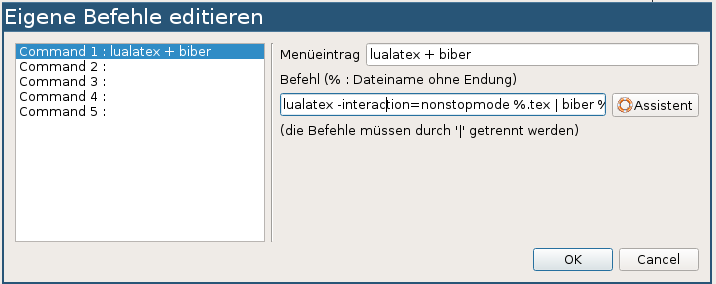
\includegraphics[width=12cm]{Plots/texmaker.png}
    \caption{Screenshot zur Erstellung des Kompilier-Befehls in Texmaker}
    \label{fig:texmaker}
\end{figure}


In Abbildung \ref{fig:texmaker} ist ein Screenshot des Befehlsmenü gezeigt. Ihren Befehl können Sie nun im Drop-Down-Menü zum 
Kompilieren des Dokuments auswählen und mit einem Klick auf den Pfeil starten.

\subsection{Aufräumen}

Nach einem \LaTeX-Fehler ist es oft notwendig, die erstellten Hilfsdateien zu löschen.
Klicken Sie hierzu auf \emph{Werkzeuge}→\emph{Aufräumen}.


\chapter{\LaTeX-Grundlagen}

Bitte beachten Sie beim Schreiben der Arbeit folgende Konventionen bzw. Grundlagen:

\begin{itemize}
    \item \textbf{Abschnitte und Zeilenumbrüche} \\
        Es sollten im Fließtext keine Zeilenumbrüche mit \textbackslash\textbackslash \ erzwungen werden.
        Schreiben Sie höchsten einen Satz in eine Code-Zeile.
        Absätze werden im Code mit einer Leerzeile markiert und dann entsprechend der Einstellung von \texttt{parskip} in der Dokumentenklasse gesetzt.
    \item \textbf{Kursiv/Aufrecht} \\
        \begin{itemize}
            \item Variablen und physikalische Größen werden kursiv gesetzt. 
            \item Einheiten werden immer aufrecht und mit einem halben Leerzeichen Abstand zur Zahl gesetzt. Nutzen Sie \texttt{siunitx}!
            \item Mathematische Konstanten und Funktionen werden ebenfalls aufrecht gesetzt. Zum Beispiel die Eulersche Zahl e, das imaginäre i und das infinitesimale d.
                Im Mathematikmodus können Sie dies mit dem Befehl \verb_\mathrm{}_ erreichen. Für die Funktionen stellt \LaTeX \ Befehle bereit, z.B. \verb+\arccos+.
            \item Integrand und ein $\mathrm{d}x$ sollten ebenfalls durch ein kleines Leerzeichen (\verb+\,+) getrennt werden.
        \end{itemize}
        


\end{itemize}

\section{Zahlen und Einheiten}

Jede Zahl, jede Einheit und jede Zahl mit Einheit sollte mit Hilfe der in dem Paket \texttt{siunitx} zur Verfügung gestellten Befehle gesetzt werden.
Grundsätzlich gilt: Einheiten werden aufrecht gesetzt und haben ein kleines Leerzeichen (\verb+\,+) Abstand zu ihrer Zahl. 
Werden Fließkommazahlen ohne \texttt{siunitx} gesetzt, entsteht ein hässlicher Leerraum zwischen Komma und erster Nachkommastelle, da \LaTeX \ das Komma nicht als Dezimaltrennzeichen, sondern als Satzzeichen interpretiert.

Das Paket wurde mit deutschen Spracheinstellungen (also mit Komma als Dezimaltrennzeichen und $\cdot$ zwischen Zahl und Zehnerpotenz) geladen, sowie mit den Einstellungen, dass die Standardabweichung stets durch $\pm$ abgetrennt wird und Einheiten falls nötig als Brüche ausgegeben werden.

\begin{table}
    \centering
    \caption{Beispiele für siunitx}
    \label{tab:si}
    \begin{tabular}{l r}
        \toprule
        Befehl     &   Ergebnis \\
        \midrule
        \verb+\num{1.2345}+ & \num{1.2345} \\
        \verb+\num{1.2e3}+ & \num{1.2e3} \\
        \verb_\num{1.2 +- 0.2}_ & \num{1.2+-0.2} \\
        \verb+\num{10000}+ & \num{10000} \\
        \verb+\si{\meter\per\second}+ & \si{\meter\per\second} \\
        \verb+\SI{1.2(1)}{\micro\ampere}+ & \SI{1.2(1)}{\micro\ampere} \\
        \verb+\SI{1.2\pm0.1e3}{\kilo\gram\per\cubic\meter}+ & \SI{1.2\pm0.1e3}{\kilo\gram\per\cubic\meter} \\
        \bottomrule 
    \end{tabular}
\end{table}

Das Paket stellt unter anderem die drei wichtigen Befehle
\begin{itemize}
    \item \texttt{\textbackslash num\{Zahl\}},
    \item \texttt{\textbackslash si\{Einheit\}} und
    \item \texttt{\textbackslash SI\{Zahl\}\{Einheit\}}
\end{itemize}
zur Verfügung.
Diese Befehle sollten stets genutzt werden, wenn Zahlen angegeben werden. 
Sie funktionieren sowohl im Text- als auch im Mathematikmodus.
In Tabelle \ref{tab:si} sind einige Beispiele aufgetragen. Bitte lesen Sie die Dokumentation \cite{siunitx}.

\section{Das Literaturverzeichnis}

Das Literaturverzeichnis wird mit Hilfe von BibLaTeX und biber erstellt.
Tragen Sie alle ihre Quellen in die Datei \texttt{references.bib} ein, Sie enthält bereits
einige Beispiele. Für weitere Informationen lesen Sie bitte die Dokumentation \cite{biblatex}.

Im Text können Sie mit \verb_\cite{kürzel}_ zitieren. Seitenzahlen geben Sie in eckigen Klammern an:
\verb_\cite[10]{kürzel}_. 

Das Literaturverzeichnis ist so eingestellt, dass es Ihre Quellen in alphabetischer Reihenfolge nach Autoren nummeriert.
Möchten Sie das Literaturverzeichnis nach der Reihenfolge des Auftauchens im Text sortieren, fügen sie die Paktetoption \texttt{sorting=none} beim Laden
des BibLaTeX-Pakets hinzu.

Den Zitier- und Bibliographie-Stil geben sie mit der Option \texttt{style=Stil} an. Die beiden gebräuchlisten Stile sind \texttt{numeric} und \texttt{alphabetic}. 
Bei \texttt{numeric} werden die Quellen durchnummeriert, bei \texttt{alphabetic} wird ein Buchstabenkürzel aus Autor(en)-Name(n) und Jahr verwendet.
Für weitere Stile konsultieren Sie bitte die Dokumentation: \cite{biblatex}.

Ein Beispiel für das Zitieren eines Buches lautet so \cite{handbook_adhesives},
wissenschaftliche Artikel hingegen werden so \cite{einstein} zitiert.

Damit das Literaturverzeichnis erstellt wird, ist ein Aufruf von \texttt{biber} nach einem ersten kompilieren mit \texttt{lualatex} nötig.
Danach muss das Dokument erneut mit \texttt{lualatex} kompiliert werden. 

Zum korrekten Kompilieren des Dokuments siehe Kapitel \ref{make}.

\chapter{Abbildungen und Tabellen}

\section{Abbildungen}

Achten Sie bei ihren Plots auf ausreichend große Achsenbschriftungen, ausreichende Schriftdicken und gut unterscheidbare Farben.
Im Idealfall haben Sie im Plot und der Arbeit die gleiche Schriftgröße und Schriftart.
Dies lässt sich durch Erstellen des Plots in der korrekten Größe und Einbinden mit dem optionalen Argument \texttt{scale=1} erreichen. Ein Beispiel sehen Sie in Abbildung \ref{fig:bsp}.

Nutzen Sie wenn möglich Vektorgrafiken (pdf) und nur in Ausnahmen Rastergrafiken wie .png oder .jpg.
Setzen Sie Punkte hinter Abbildungsunterschriften.

\begin{figure}
    \centering
    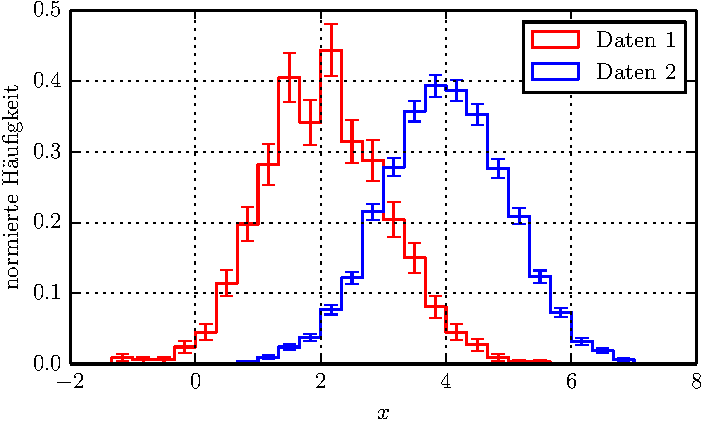
\includegraphics[scale=1]{./Plots/Histogramm.pdf}
    \caption{Ein Histogramm mit Fehlerbalken für zwei Datensätze, Schriftgröße und -art entsprechen der des Dokuments.}
    \label{fig:bsp}
\end{figure}

\section{Tabellen}

Tabellen sollten so einfach wie möglich aufgebaut sein, verzichten Sie auf zu viele Linien. In fast allen Fällen reichen drei horizontale Linien aus, jeweils über und unter der Tabelle und zwischen den Spaltenüberschriften und der eigentlichen Tabelle.

Das Paket \texttt{booktabs} stellt hierfür \verb_\toprule_, \verb_\midrule_ und 
\verb_\bottomrule_ zur Verfügung.
Das Paket \texttt{siunitx} stellt eine extrem mächtige neue Spalteneinstellung bereit: \texttt{S}, mit ihr können Zahlen und Einheiten sehr sauber und gut ausgerichtet gesetzt werden.

Diese Vorlage geht von Tabellenüberschriften aus, möchten Sie dagegen Tabellenunterschriften entfernen Sie das entsprechende optionale Argument für die Dokumentenklasse in der Präambel.

Ein Beispiel ist Tabelle~\ref{tab:bsp}.
\begin{table}
    \centering
    \caption{Beispieltabelle mit willkürlichen Werten, für die Zahlenwerte wurde die S-Option aus \texttt{siunitx} verwendet.}
    \label{tab:bsp}
    \begin{tabular}{S[table-format=4.2] S[table-format=3.2]}
        \toprule
        {$p \mathrel{/} \si{\pascal}$}  & {$T \mathrel{/} \si{\kelvin}$} \\
        \midrule
        1024,23 & 273,15 \\
        1025,31 & 274,5 \\
        1026,27 & 276,2 \\
        \bottomrule
    \end{tabular}
\end{table}


\appendix
% Hier beginnt der Anhang, nummeriert in lateinischen Buchstaben
\chapter{Ein Anhangskapitel}

Hier könnte ein Anhang stehen, falls Sie z.\,B.\ Code, Konstruktionszeichnungen oder Ähnliches mit in die Arbeit bringen wollen.
Im Normalfall stehen jedoch alle Ihre Resultate im Hauptteil der Bachelorarbeit und ein Anhang ist überflüssig.

\section{Einkristalloberflächen}
        Die geordneten Strukturen eines Einkristalls kommen durch die Wechselwirkung der Elektronen zwischen den einzelnen Atomen.
        So ergibt sich eine periodische Anordnung der Atome im thermischen Gleichgewicht.
        Dabei sind die Atome nicht komplett starr an ihre Plätze gebunden, sondern führen kleine Schwingungen um diesen aus.
        Mit der Temperatur sinkt auch die Auslenkung.
        Dieses Wechselspiel der strukturellen Ordnung findet sich auch in der elektronischen Struktur wieder.
                
        Wird ein Einkristall entlang einer Kristalleben durchschnitten so ergibt sich eine Oberfläche.
        Die Ebene erhält den Namen der Indizes des auf ihr senkrecht stehenden Gittervektors $r_{hkl}$, also $(hkl)$.
        Als Oberfläche werden die oberen Atomlagen definiert, die sich in der geometrischen und/oder chemischen Art von der des Volumens unterscheiden~\cite{Fauster}.
        Aufgrund der nun fehlenden Bindungen nach oben ergeben sich neue elektronische und geometrische Eigenschaften.
        So kann es zu lateralen und transversalen Verschiebungen gegenüber der volumenartigen Struktur, so genannte Rekonstruktionen und Relaxation kommen.
        Dabei ordnen sich die Atome um, um damit einen energetisch günstigeren Zustand zu erhalten.
    
        Wie im Volumenkristall kann die Oberfläche durch eins von fünf Bravais-Gittern beschrieben werden, wobei auf jedem Gitterpunkt eine atomare Basis gesetzt wird.
        Die Punkte dieses zweidimesionalen Gitters lassen sich durch den Gittervektor
        \begin{equation}
            \vec{r}_{nm} = n \vec{a}_1 + m \vec{a}_2
            \label{eqn:Gittervek}
        \end{equation}
        mit $n,m \in \mathbb{Z}$ und den Vektoren der Einheitszelle $\vec{a}_1, \vec{a}_2$ beschreiben.
        Geimeinsam legt das Bravais-Gitter und die atomare Basis die Symmetrien der Oberfläche fest.
    
        Durch die Anlagerung von Adsorbaten können Symmetrien der Oberfläche verloren gehen.
        Die Struktur der Adsorbate relativ zur Oberfläche wird Überstruktur genannt.
        Durch den meist größeren Abstand der Adsorbate untereinander als der Basen des Substrates ergibt sich auch eine größere Einheitszelle.
        Beim Schneiden der Einkristalle um eine Oberfläche zu erhalten können sich unter anderem auch Stufen ausbilden.
        Vermehrt treten diese Stufen bei hochindizierten Oberflächen auf, wobei einzelne Terrassen dann eine niedrigindizierte Oberfläche darstellen~\cite{Fauster}.
        Diese Stufen oder auch Defekte in der Oberfläche bilden Keimzellen für Anlagerung von Adsorbaten.
        Um die Überstruktur des Adsorbate zu beschreiben wird die von ihnen aufgespannte Einheitszelle aus den Gittervektoren des Substrats rekosntruiert.
        Die Gittervektoren des Übergitters $\vec{b}_1, \vec{b}_2$ lassen sich dann als Matrixschreibweise darstellen.
        Damit ergibt sich auch die Überstrukturmatrix $C$ mit 
        \begin{equation}
            \begin{pmatrix}
                \vec{b}_1 \\
                \vec{b}_2 \\
            \end{pmatrix}
            = 
            \begin{pmatrix}
                C_{11} & C_{12} \\
                C_{21} & C_{22} \\
            \end{pmatrix}
            \begin{pmatrix}
                \vec{a}_1 \\
                \vec{a}_2 \\
            \end{pmatrix}.
        \end{equation}
        Relative Verschiebungen zum Substrat bleiben dabei ohne Beachtung, es zeigt nur die Periodizität der Struktur an.
        Ferner kann es zur Aubildung verschiedener Domänen kommen, besonders dann, wenn die Symmetrie des Übergitters kleiner als die des Substrates ist~\cite{Fauster}.
        Einzelne Domänen weisen Symmetrie äquivalente Anordnungen auf, häufug handelt es sich nur umgedrehte Einheitszellen.
        Nicht nur Adsorbatebedeckungen lassen sich durch diese Notation beschreiben, auch die Rekonstruktion der Oberfläche.
        Hierbei sind es keine Adsorbatatome, sondern die Oberflächenatome selbst, die eine neue Struktur ausbilden.
        Die Relaxation, welche die Änderung im Lagenabstand beschreibt kann hingegen nicht durch dies Notation beschrieben werden.
        Sie ist ebenso wie die Rekonstruktion vom Material, der Kristallstruktur und der Oberflächenorientierung abhängig.
        Einige Rekonstruktionen und Relaxation hängen auch vom Präperationsprozess ab, wenn die Oberfläche selbst metastabil ist.
    
        Wie bereits erwähnt hängen geometrische und elektronische Struktur stark zusammen.
        Sodass sich an Oberflächen durch die fehlenden Bindungen die elektronische Struktur verändern kann.
        Die quantenmechanische Beschreibung der Elektronen erlaubt es auch die elektronischen Zustände der Oberfläche durch Quantenzahlen auszudrücken.
        Hier ist $\vec{k}_{||}$ der Wellenzahlvektor der Oberfläche die Ausschlag gebende Größe um die Oberflächenbandstruktur $E(\vec{k}_{||})$ zu beschreiben.
        Ganz besondere Beachtung erhalten die Zustände nahe der Fermikante $E_\text{F}$ die für leitenden Eigenschaften verantwortlich sind.
        Erhaltene Oberflächenbandstruktur kann von der der Volumenbandstruktur abweichen.
        Dies führt zum Teil zu Oberflächenzuständen, die unterscheiden sich energetisch von denen im Volumenkristall und können somit nur in dessen Bandlücke auftreten.
    
        % Ein wichtiger Ansatz für die periodische Struktur der Oberfläche und dessen elektronischen Zustände ist das Bloch Theorem.
        % Die Oberfläche entspricht einer Anordung äquivalenter Punkte welche durch den Gittervektor aus \autoref{eqn:Gittervek} ineinander überführt werden können

        \subsection{Eisen (100) Oberfläche}
            \begin{itemize}
                \item WKF
                \item Symmetrie - p4mm
                \item Gitterkonstante ist $a = \SI{2.862}{\angstrom}$~\cite{springer_database}
                \item bcc Struktur
            \end{itemize}
        
        \subsection{Gold (111) Oberfläche}
            Gold gehört zu den Edelmetallen und kristallisiert in der flächenzentrierten Struktur mit einer Gitterkonstanten von \SI{4.08}{\angstrom}~\cite{Marx}.
            Es ist besonders leitfähig, stabil und wenig reaktiv, dennoch rekosntruiert die Oberfläche in einer Fischgräten-Struktur ($\num{22} \times \sqrt{\num{3}}$)~\cite{5A_3}.
            Die Austrittsarbeit der (111)-Oberfläche wurde dabei auf \SI{5.46}{\electronvolt} bestimmt~\cite{5A_4}.
            Ebenfalls bildet sich auch ein sehr präsenter Oberflächenzustand aus.
            
            Auf Grund der sehr ähnlichen Gitterkonstante zu der des Nickeloxids von nur etwa \SI{2}{\percent} eignet es sich besonders gut als Substrat \cite{NiO_36}.
            \begin{itemize}
                \item Ebenenabstand in Au(111) $d_0 = \SI{2.35}{\angstrom}$.\textbf{\cite{5A_1}}
            \end{itemize}

            Bereits bekannt ist, dass sich auf diesem Substrat das Pentacene anordnet~\cite{5A_1, 5A_3}.
            Die lange Molekülachse liegt dabei parallel zu den Reihen der Goldatome, mit den äußeren Ringen und somit die $\pi$-Orbitale direkt oberhalb eines Goldatoms.
            Diese Positionierung lässt auf eine starke Substrat-Molekül-Interaktion schließen~\cite{5A_3}.
            Bei der Wechselwirkung dieser handelt es sich um Physisorption, was damit auch die Adsorbate-Adsorbat-Wechselwirkung zur Formung der Einheitszelle dominieren lässt~\cite{5A_4}.
            Ferner liegen in einer Monolage flach auf der Oberfläche und einzelne Reihen sind durch eine Reihe Goldatome separiert.
            Allerdings wächst der Pentacenefilm nicht epitaxtisch, sondern in Form von Inseln mit unterschiedlichen Einheitszellen~\cite{5A_3}.

            \begin{figure}
                \centering
                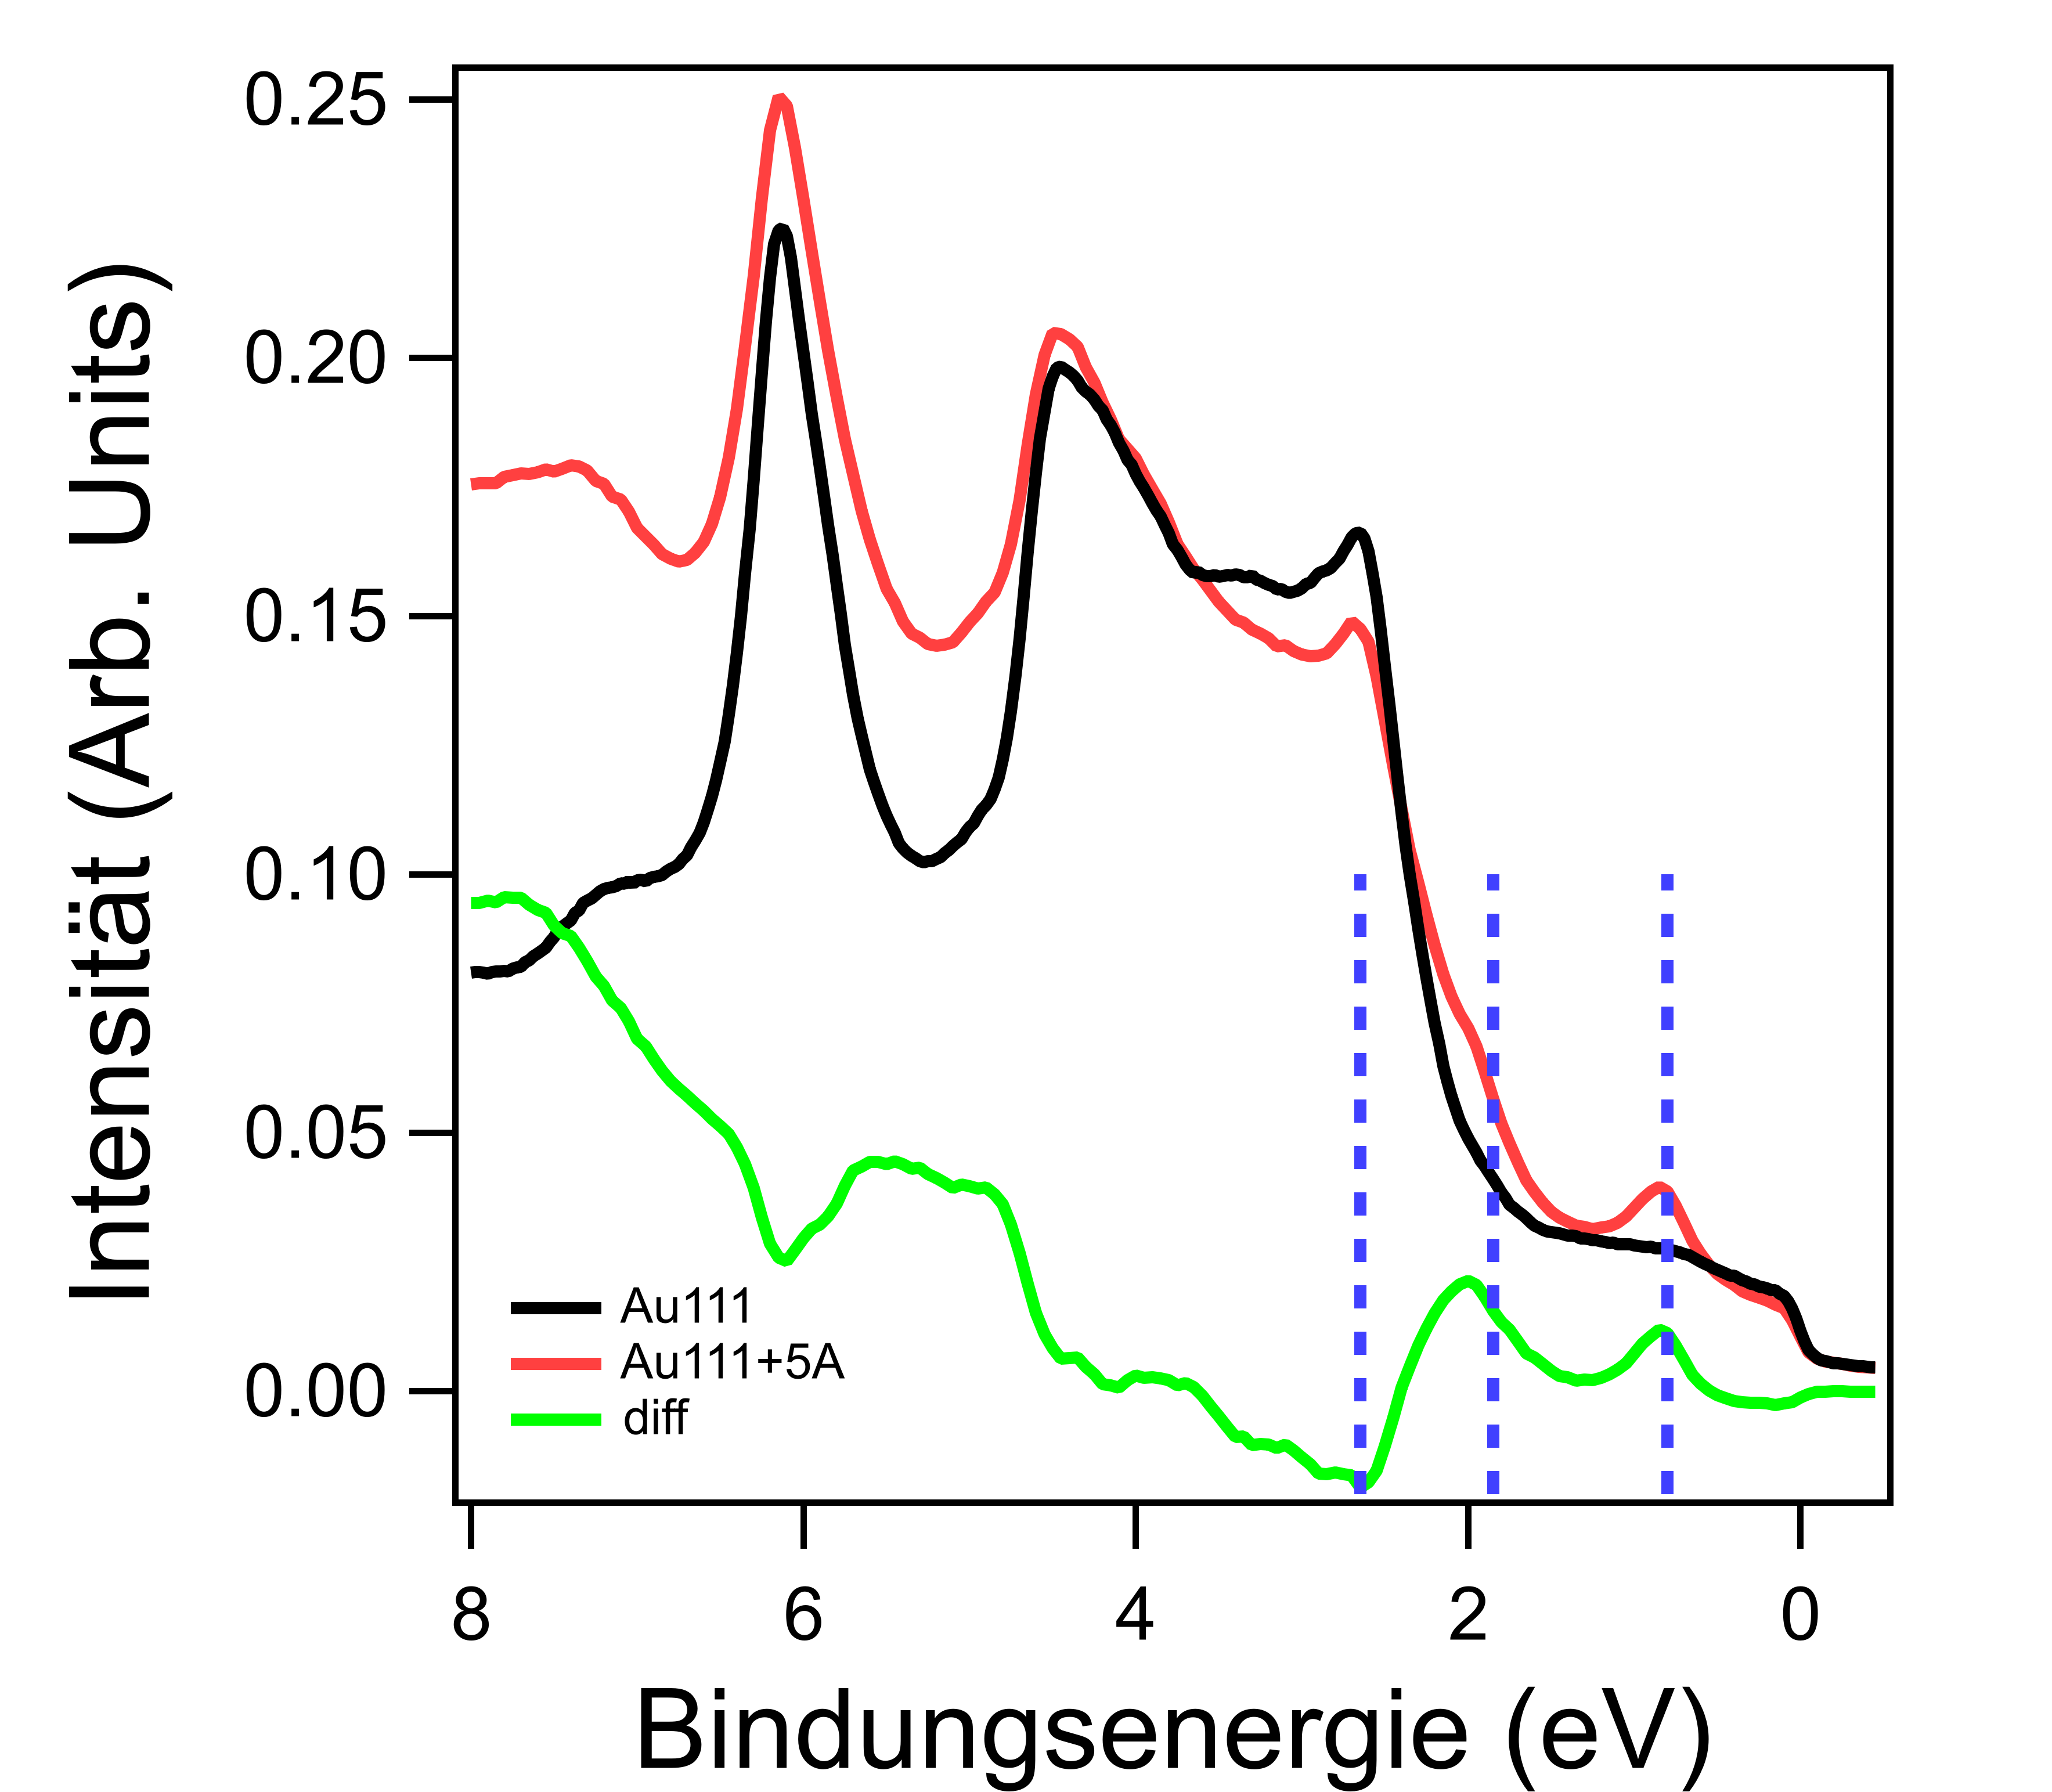
\includegraphics[width=0.5\textwidth]{Au+5A/EDC_Au_5A_mod.png}
                \caption{Die integrierten Spektren für reines Gold, Gold mit einer Monolage Pentacene und deren Differenz.}
                \label{fig:EDC_Au+5A}
            \end{figure}
            Das Goldsubstrat eignet sich ebenfalls zur Kalibrierung der Monolage von Pentacene, da bereits bekannt ist, dass sich diese flach auf der Oberfläche ordnet \cite{5A_1}.
            Bei der Wechselwirkung mit dem Substrat handelt es sich um die Physisorption durch einen Substrat-Molekülabstand von \SI{3.28}{\angstrom} \cite{5A_1}.
            % Es ergibt sich so das LEED-Bild in \autoref{fig:LEED_Au+5A}, was auch die bekannte \textbf{Überstruktur} (5A_1, 5A_5) aufweist.
            Schaut man sich das winkelintegrierte Spektrum im Bereich der Valenzzustände in \autoref{fig:EDC_Au+5A} an, so sind auch deutlich Elemente zu erkennen, die durch die Moleküle hervorgerufen werden.
            Die senkrechten Linien stellen die Punkte da, an denen Bilder mit höherer Statistik aufgenommen wurden und die später zur Molekülorbitalanalyse herangezogen werden.
    
            \begin{figure}
                \centering
                \begin{subfigure}[t]{0.48\textwidth}
                    \centering
                    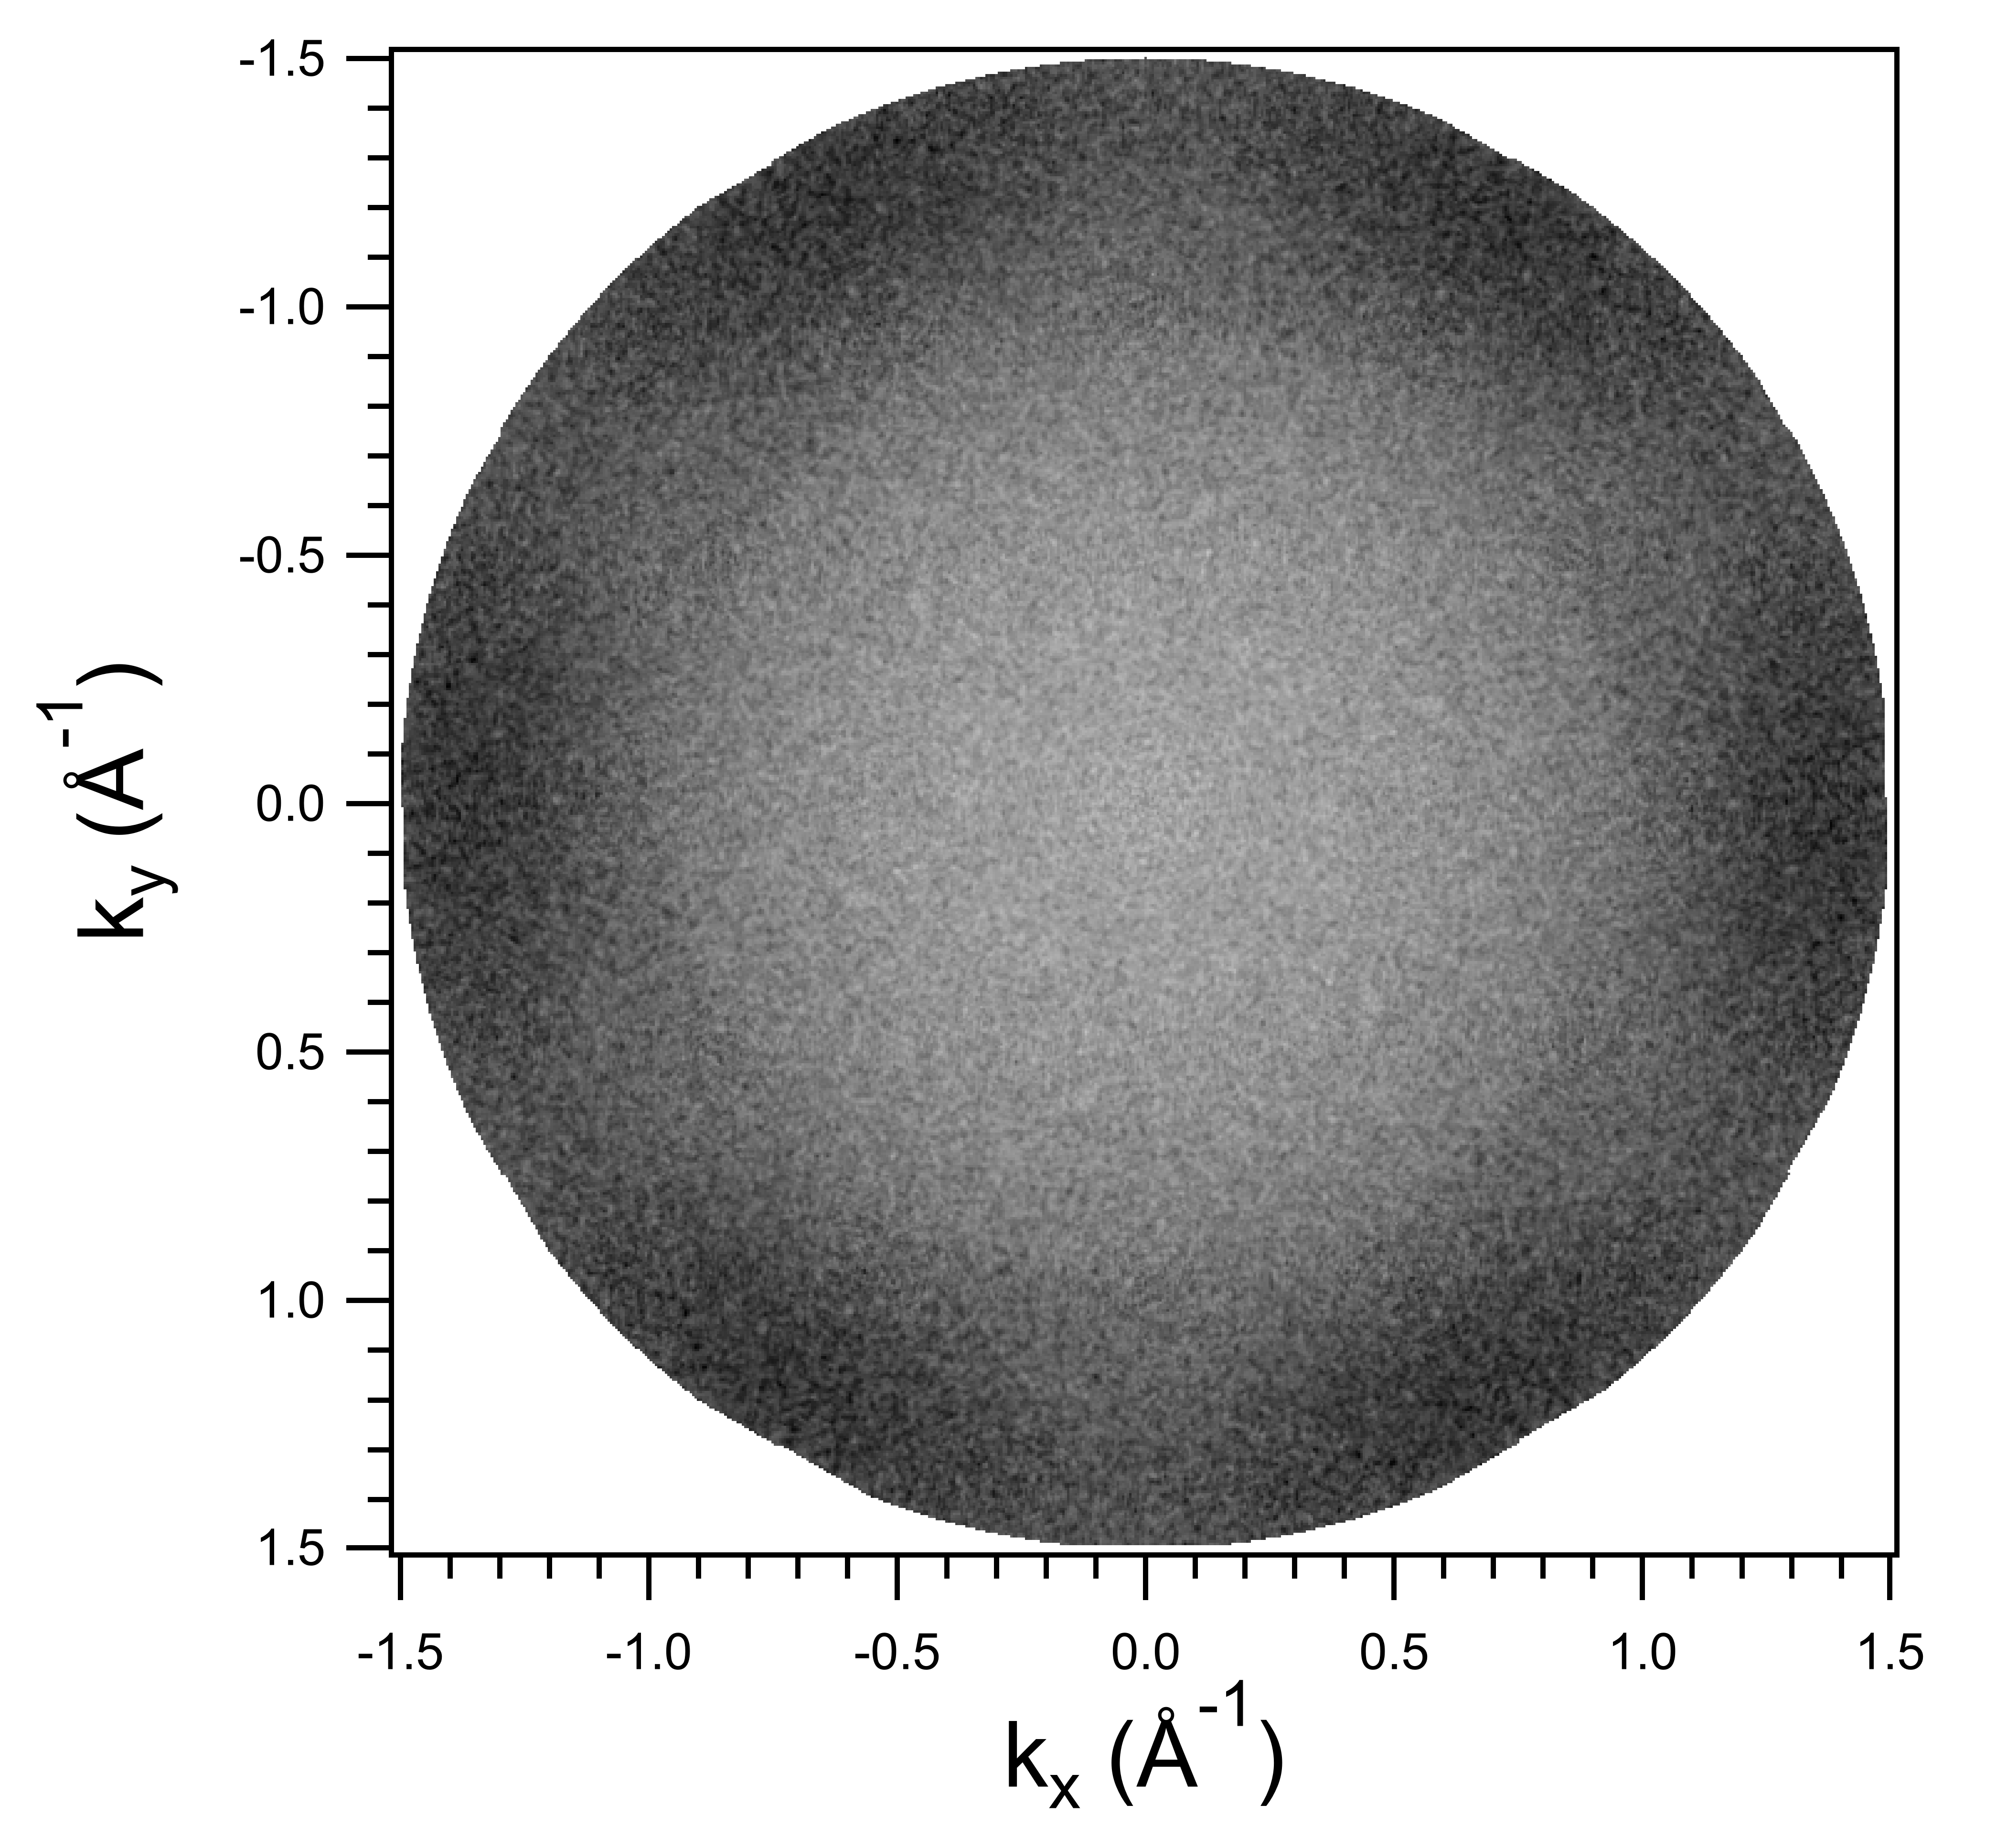
\includegraphics[height=4cm]{Au+5A/MOT_Au_5A_exp_1.png}
                    \subcaption{Gemmesen, symmetrisiertes Bild bei einer Bindungsenergie von \SI{0.8}{\electronvolt}.}
                    \label{fig:MOT_Au+5A_exp_1}
                \end{subfigure}
                \begin{subfigure}[t]{0.48\textwidth}
                    \centering
                    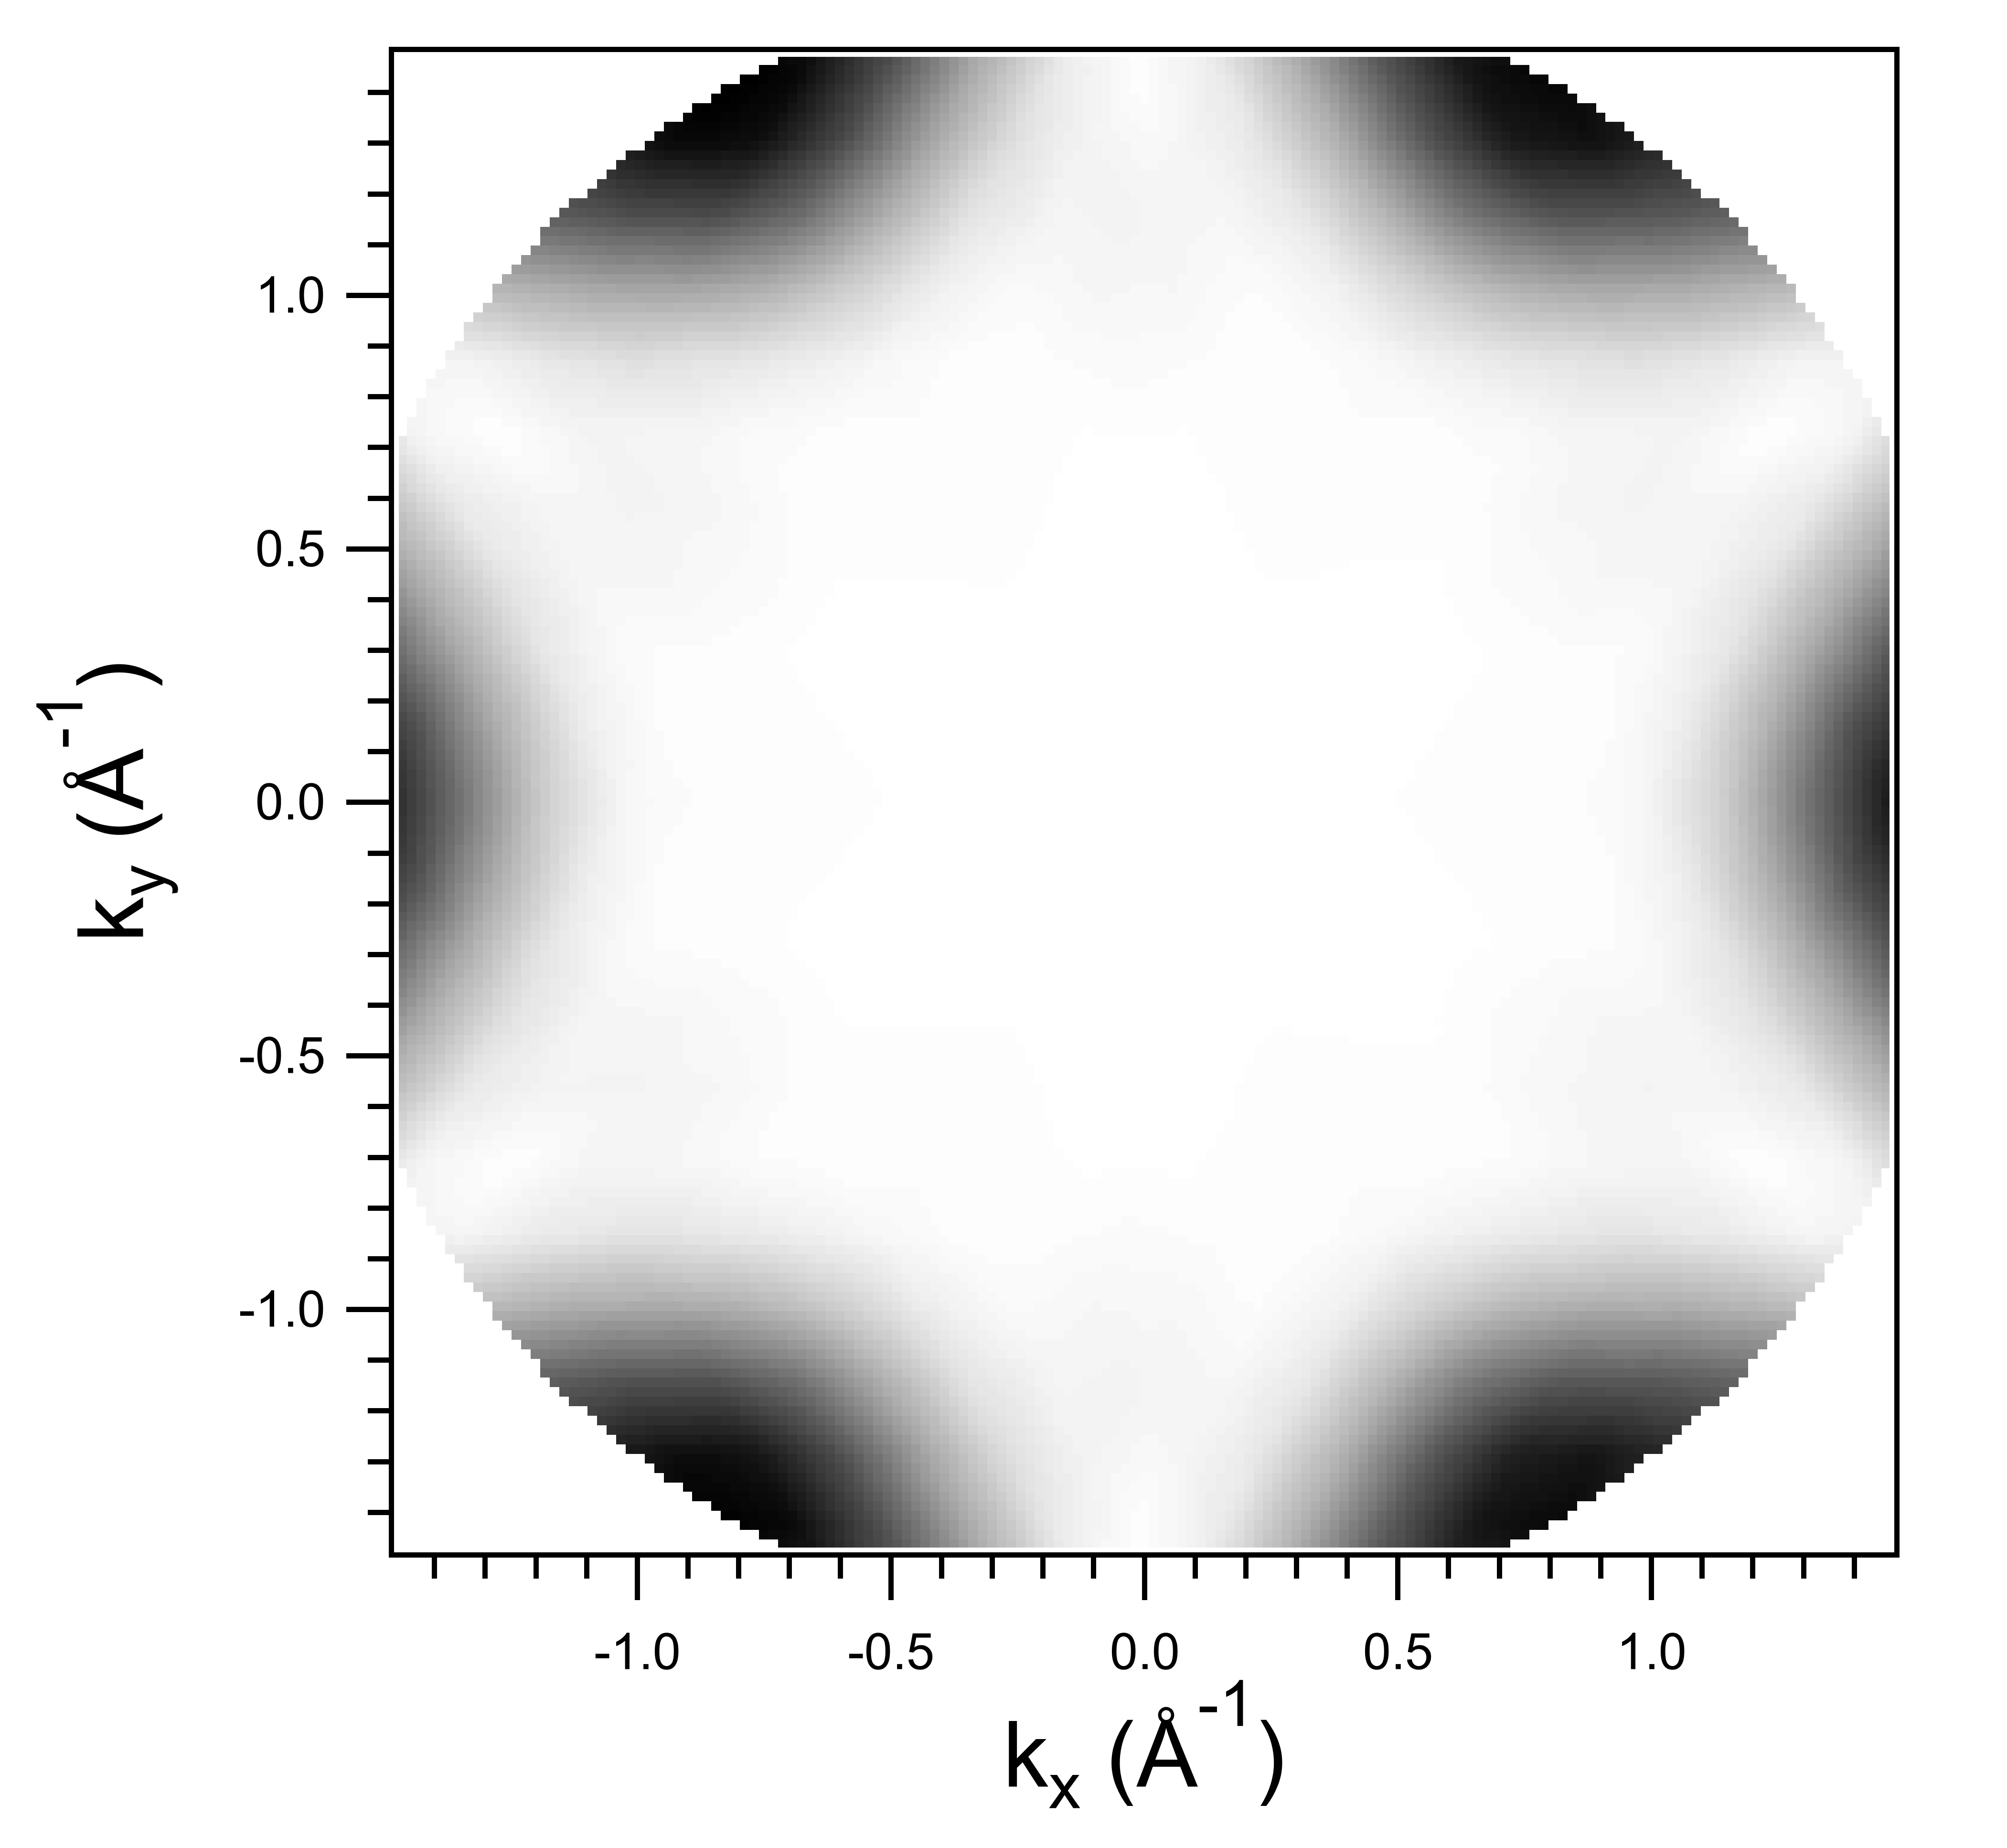
\includegraphics[height=4cm]{Au+5A/HOMO_all_CT}
                    \subcaption{Das theoretisch erwartete HOMO.}
                    \label{fig:MOT_Au+5A_theo_1}
                \end{subfigure}
                \centering
                \begin{subfigure}[t]{0.48\textwidth}
                    \centering
                    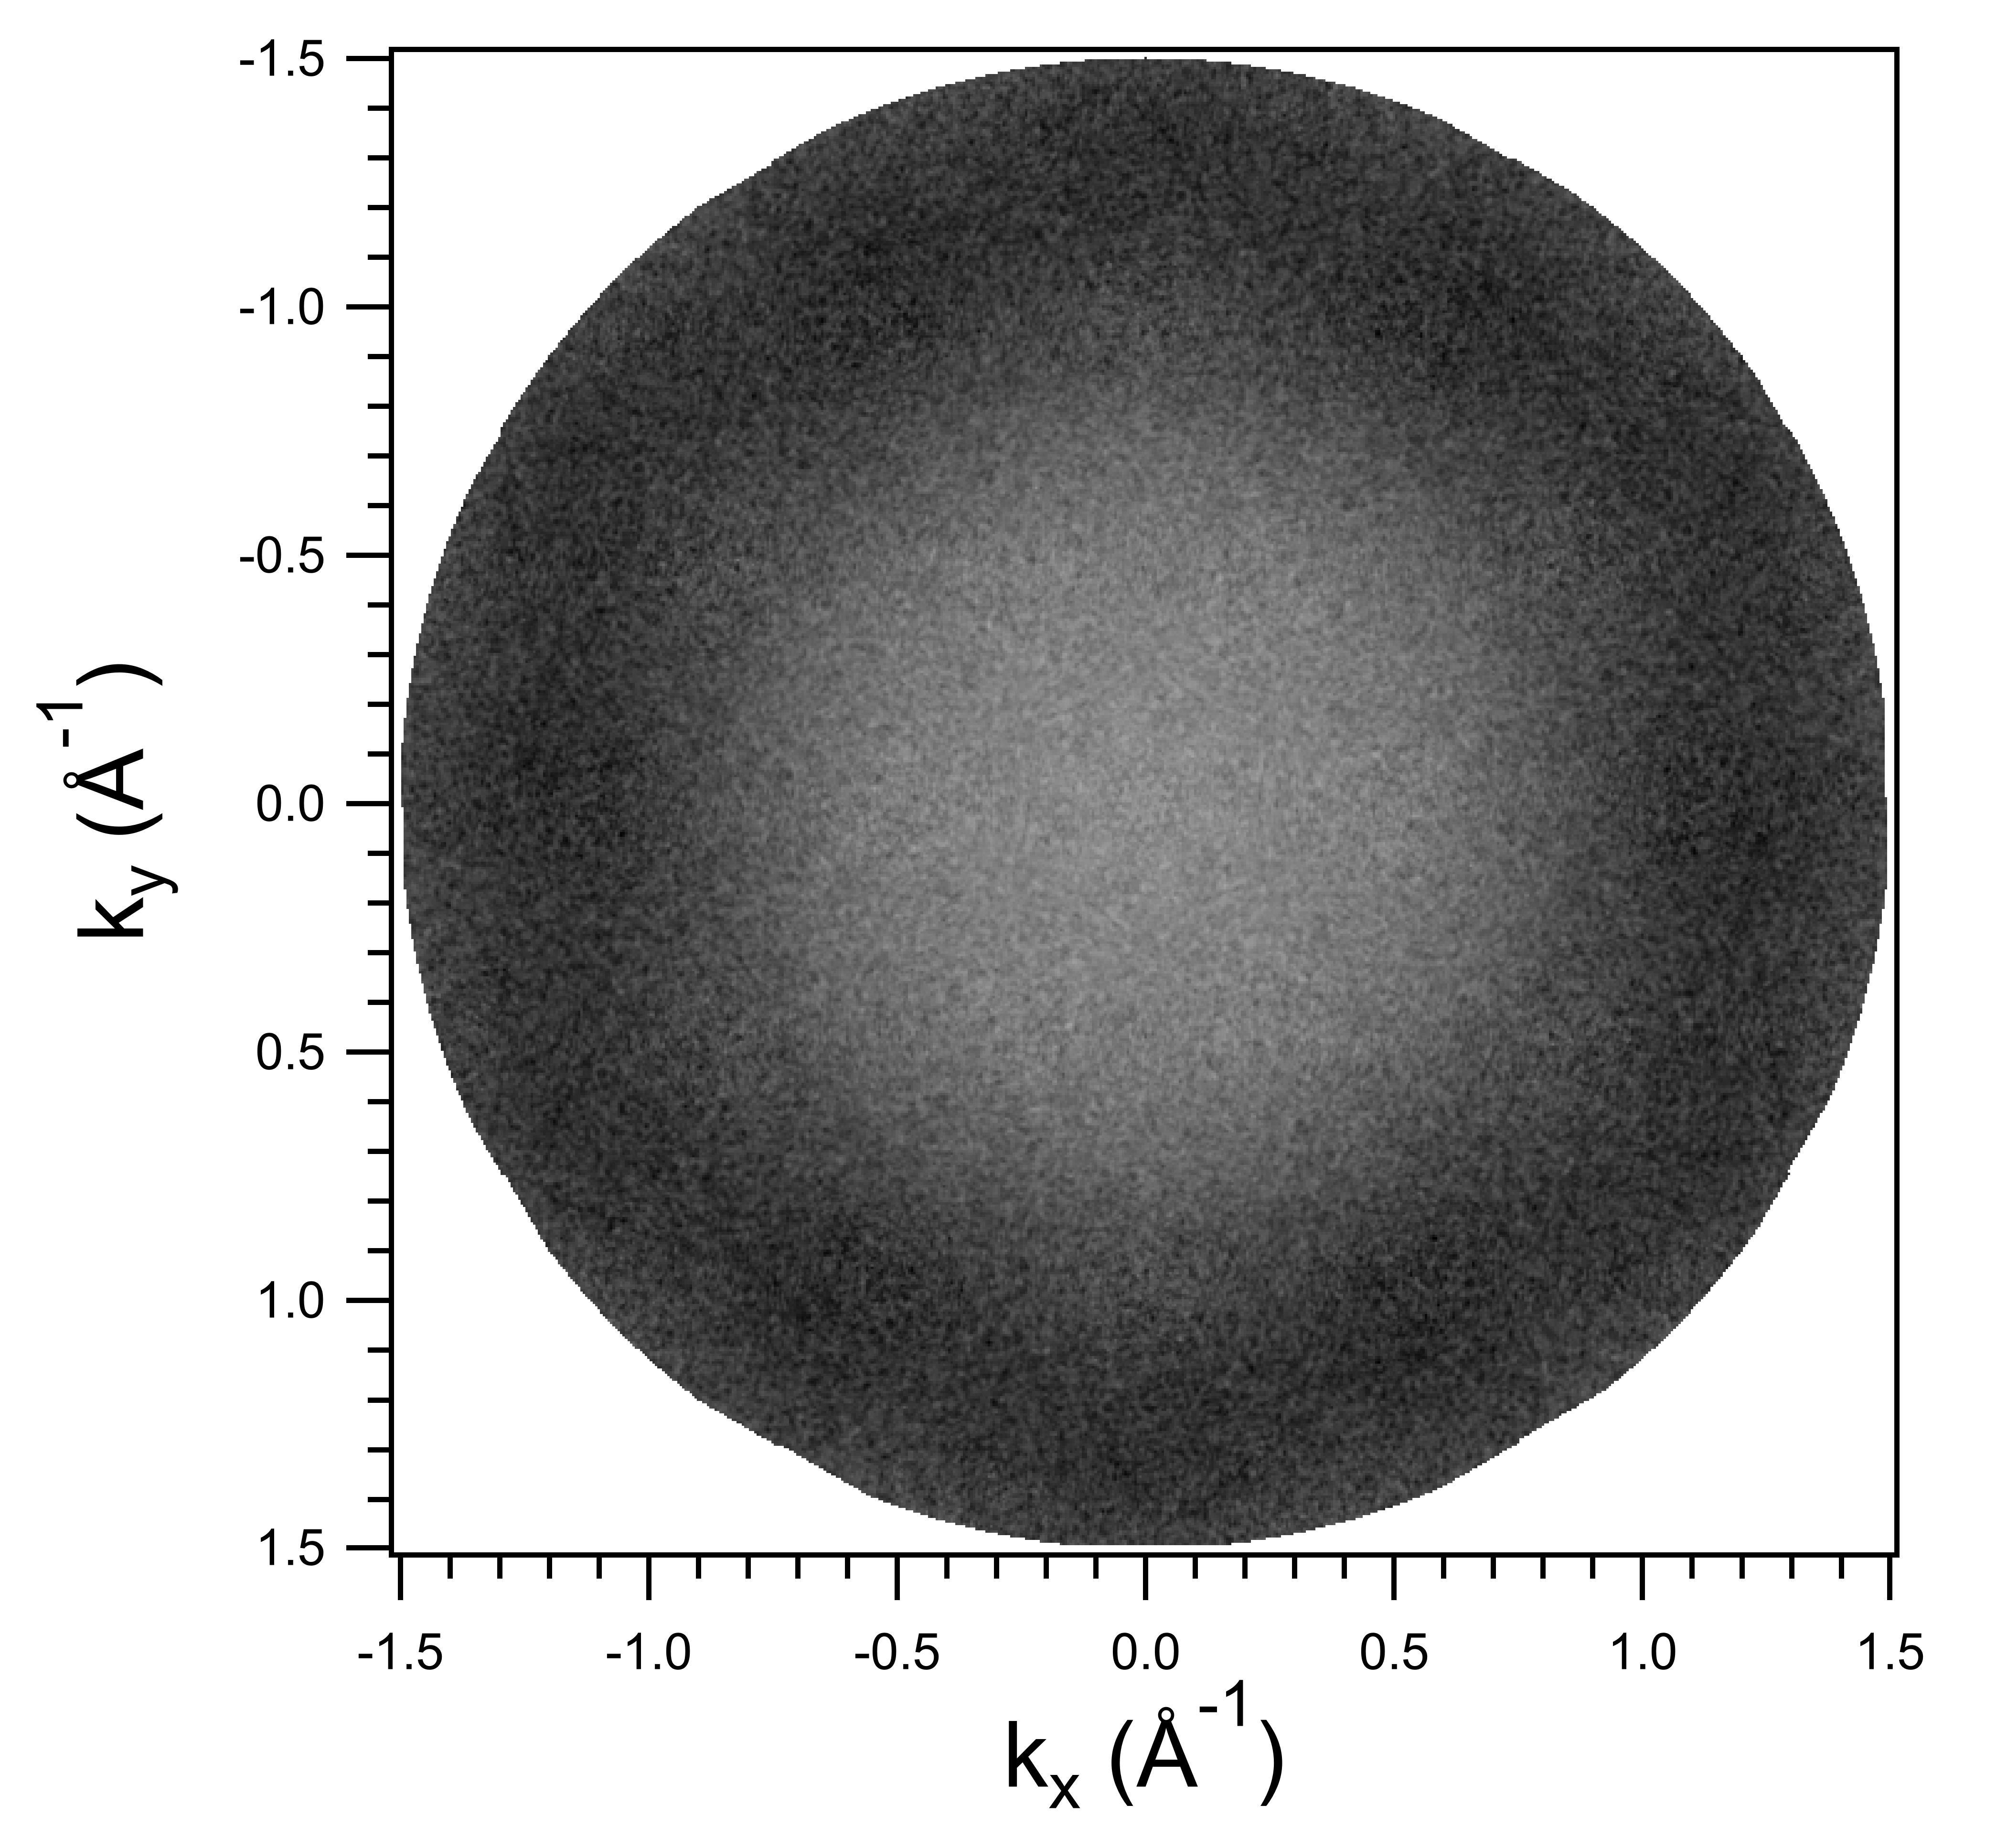
\includegraphics[height=4cm]{Au+5A/MOT_Au_5A_exp_2.png}
                    \subcaption{Gemmesen, symmetrisiertes Bild bei einer Bindungsenergie von \SI{1.85}{\electronvolt}.}
                    \label{fig:MOT_Au+5A_exp_2}
                \end{subfigure}
                \begin{subfigure}[t]{0.48\textwidth}
                    \centering
                    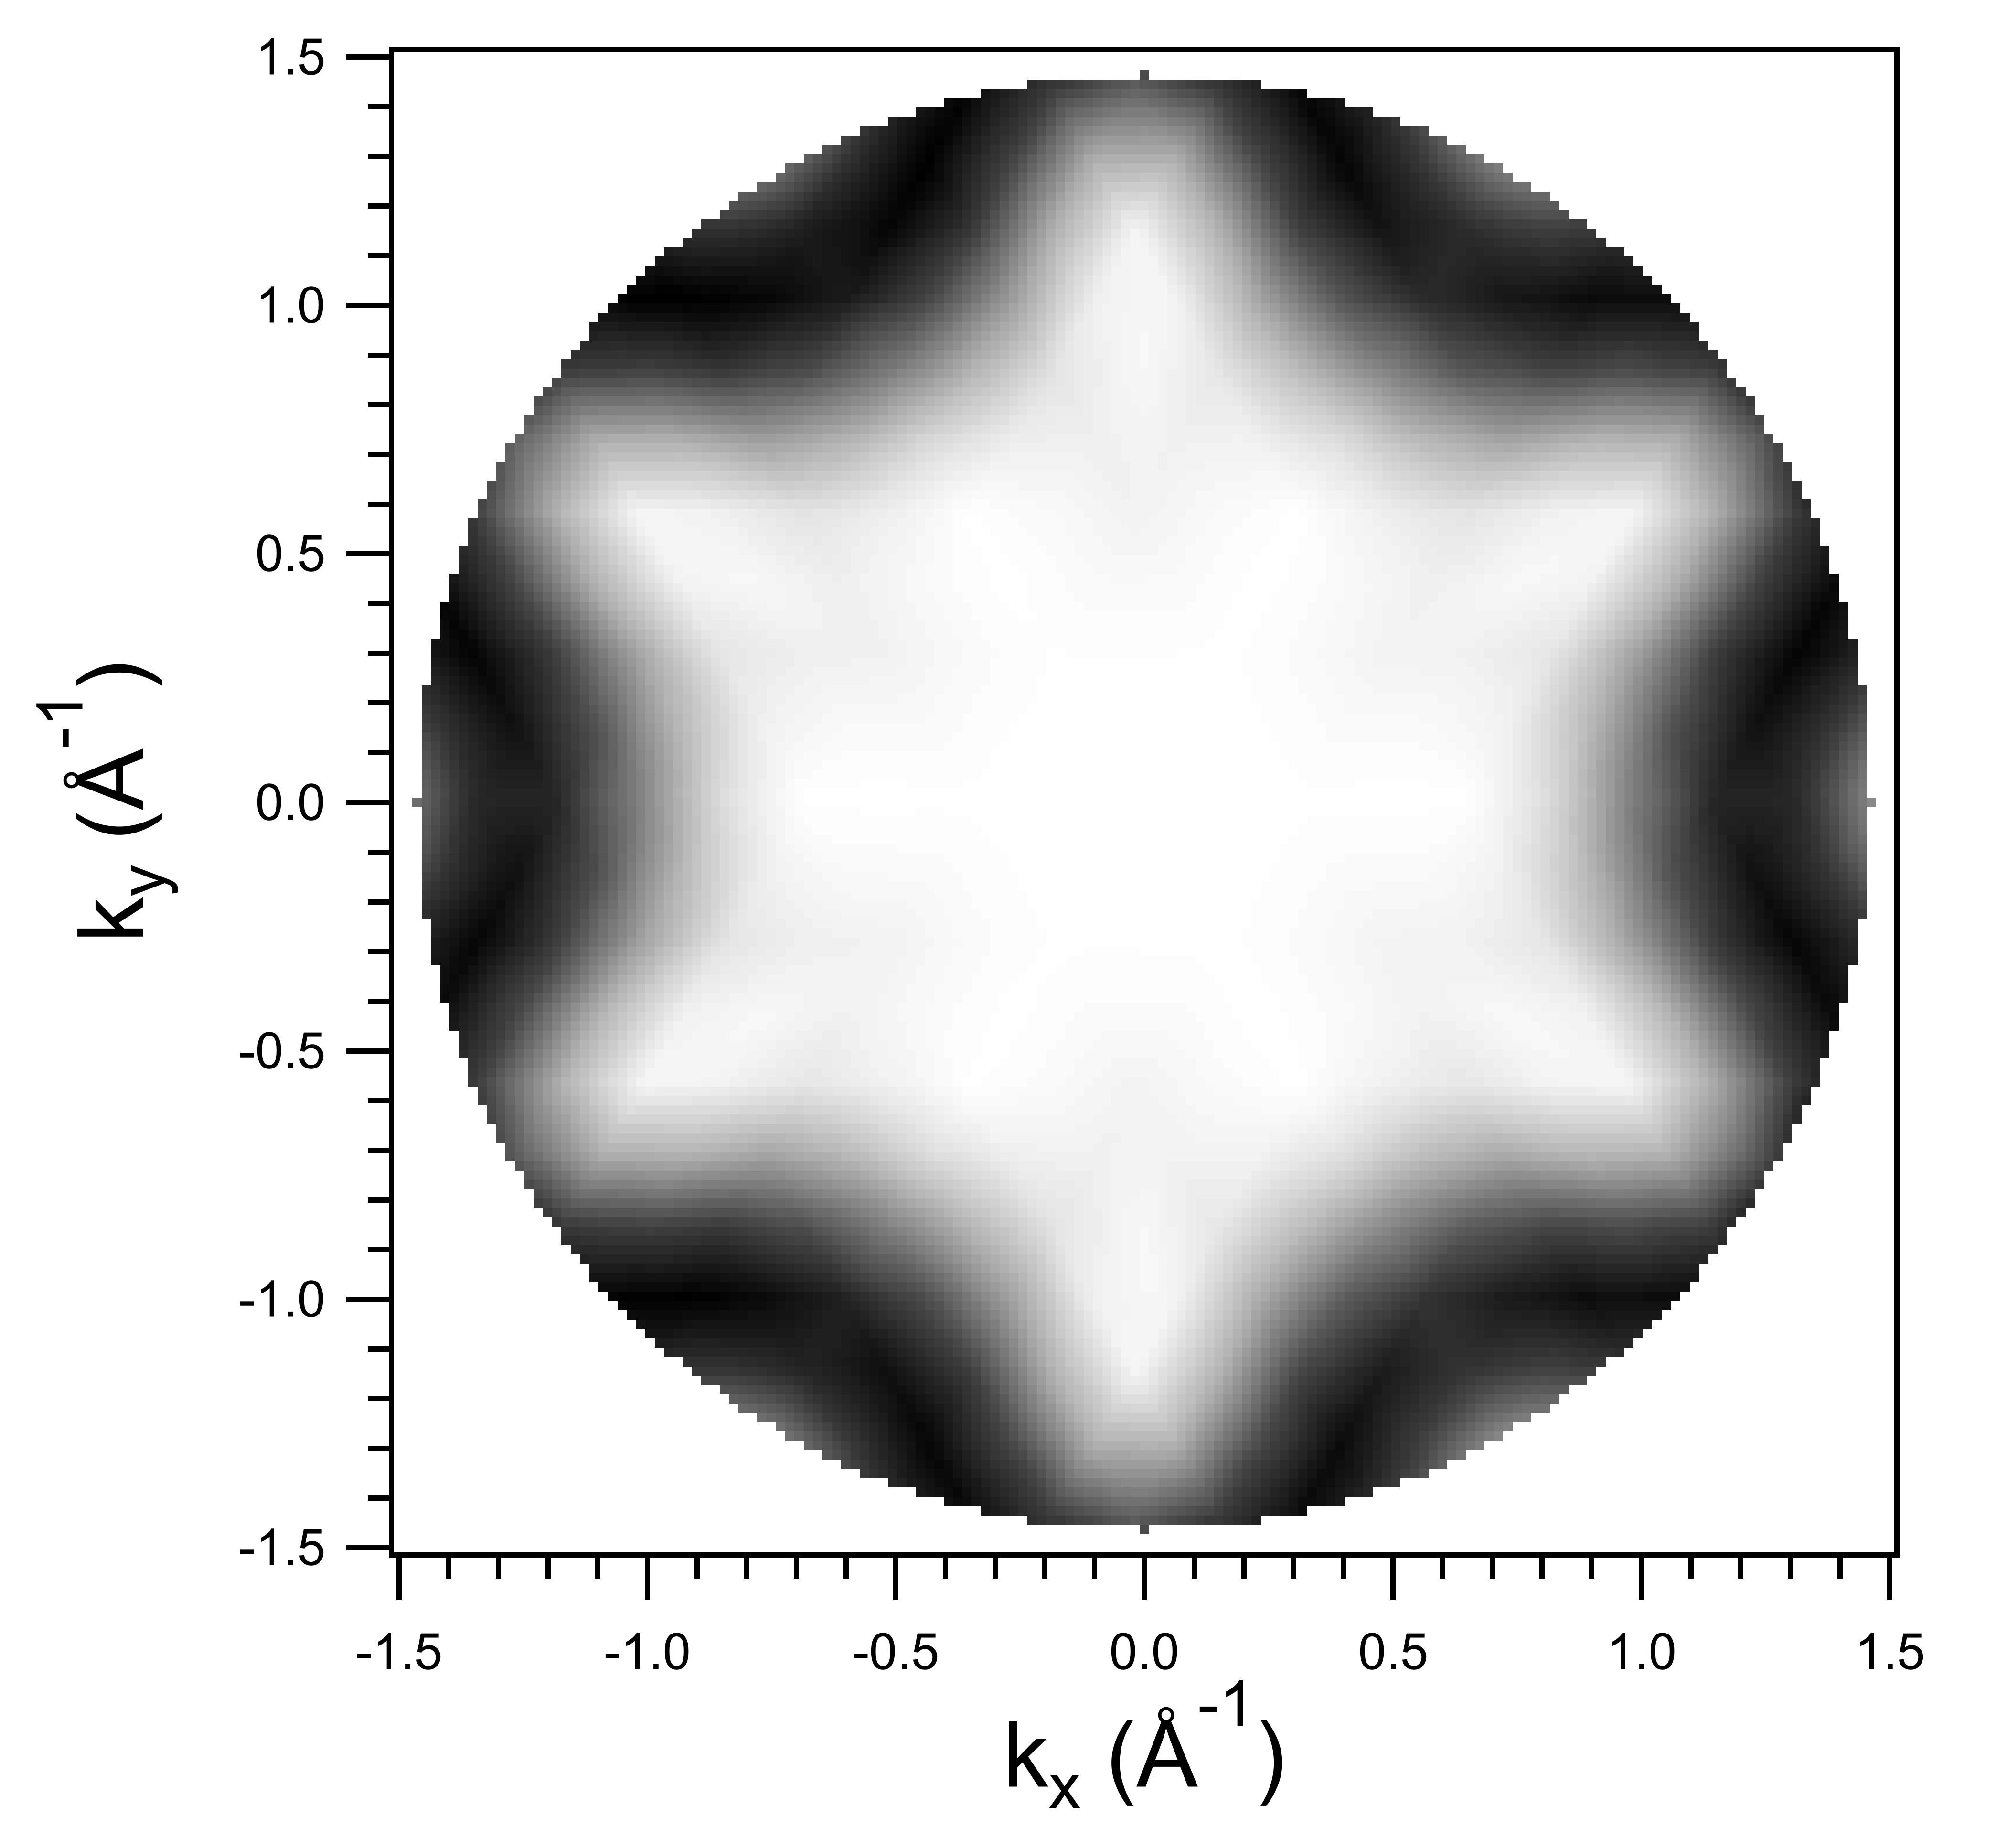
\includegraphics[height=4cm]{Au+5A/HOMO1_all_CT}
                    \subcaption{Theorie Oribtale mit Symmetrisierung des HOMO-1.}
                    \label{fig:MOT_Au+5A_theo_2}
                \end{subfigure}
                \begin{subfigure}[t]{0.48\textwidth}
                    \centering
                    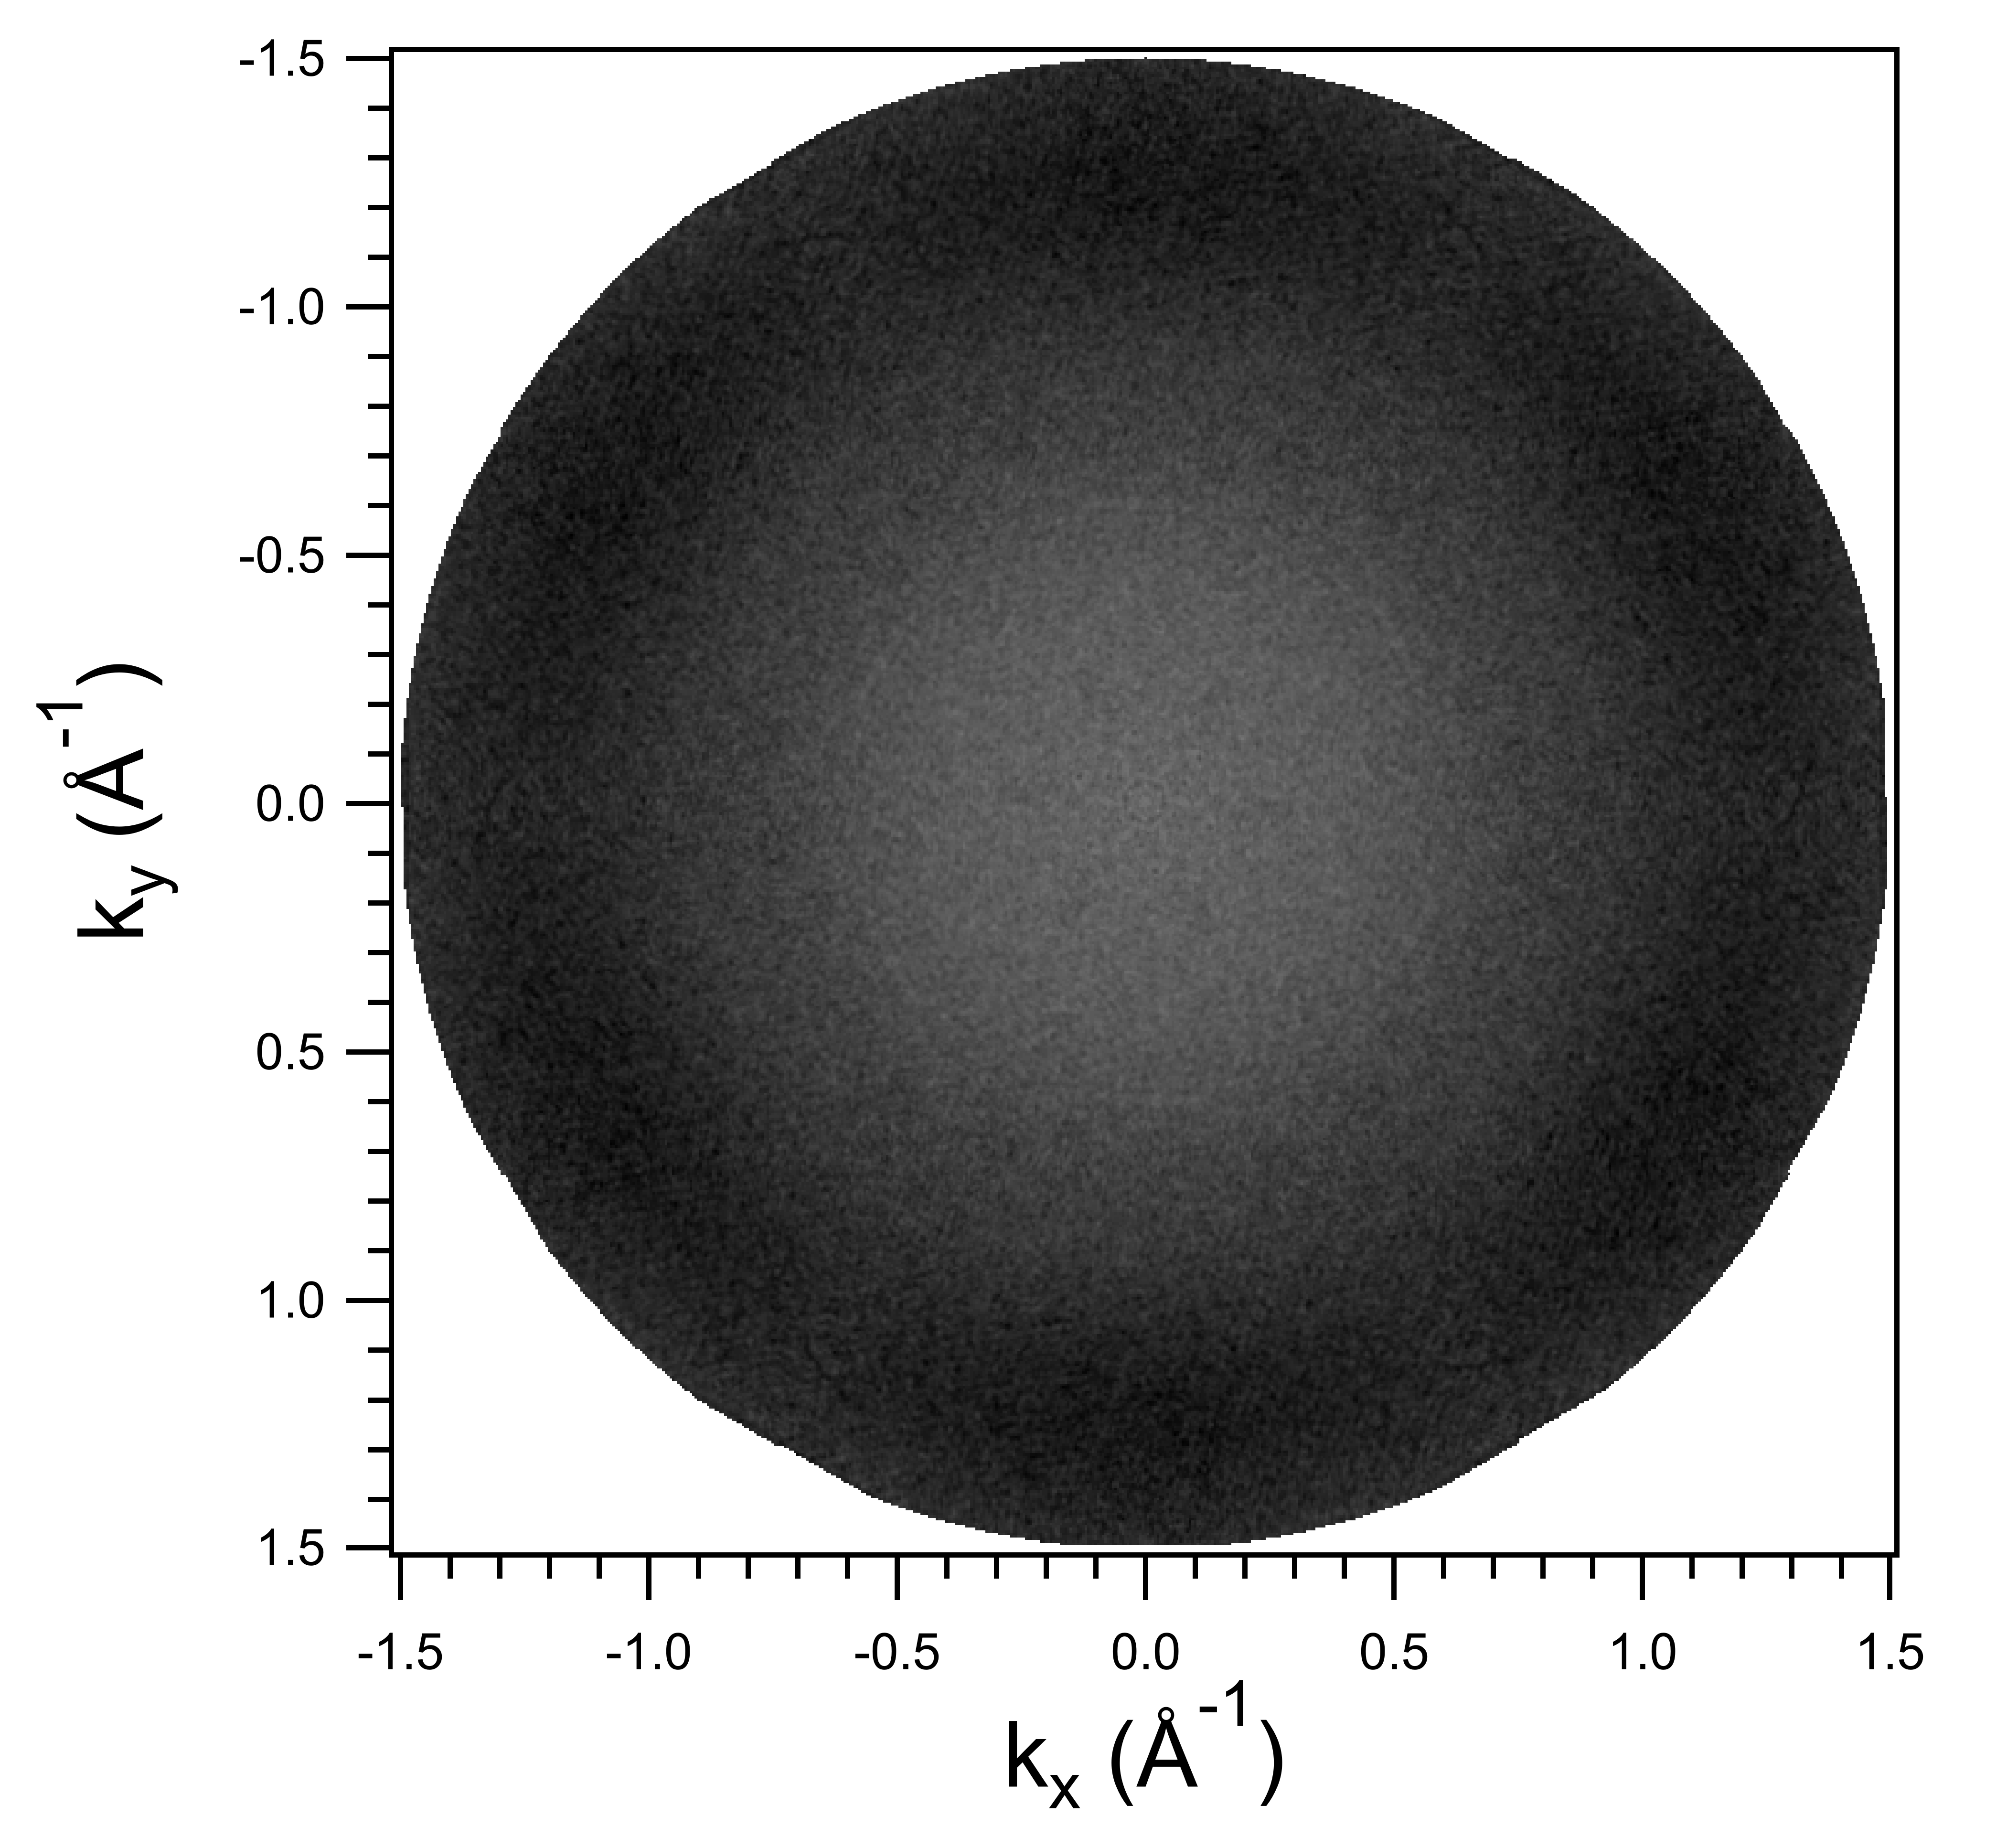
\includegraphics[height=4cm]{Au+5A/MOT_Au_5A_exp_3.png}
                    \subcaption{Gemmesen, symmetrisiertes Bild bei einer Bindungsenergie von \SI{2.65}{\electronvolt}.}
                    \label{fig:MOT_Au+5A_exp_3}
                \end{subfigure}
                \begin{subfigure}[t]{0.48\textwidth}
                    \centering
                    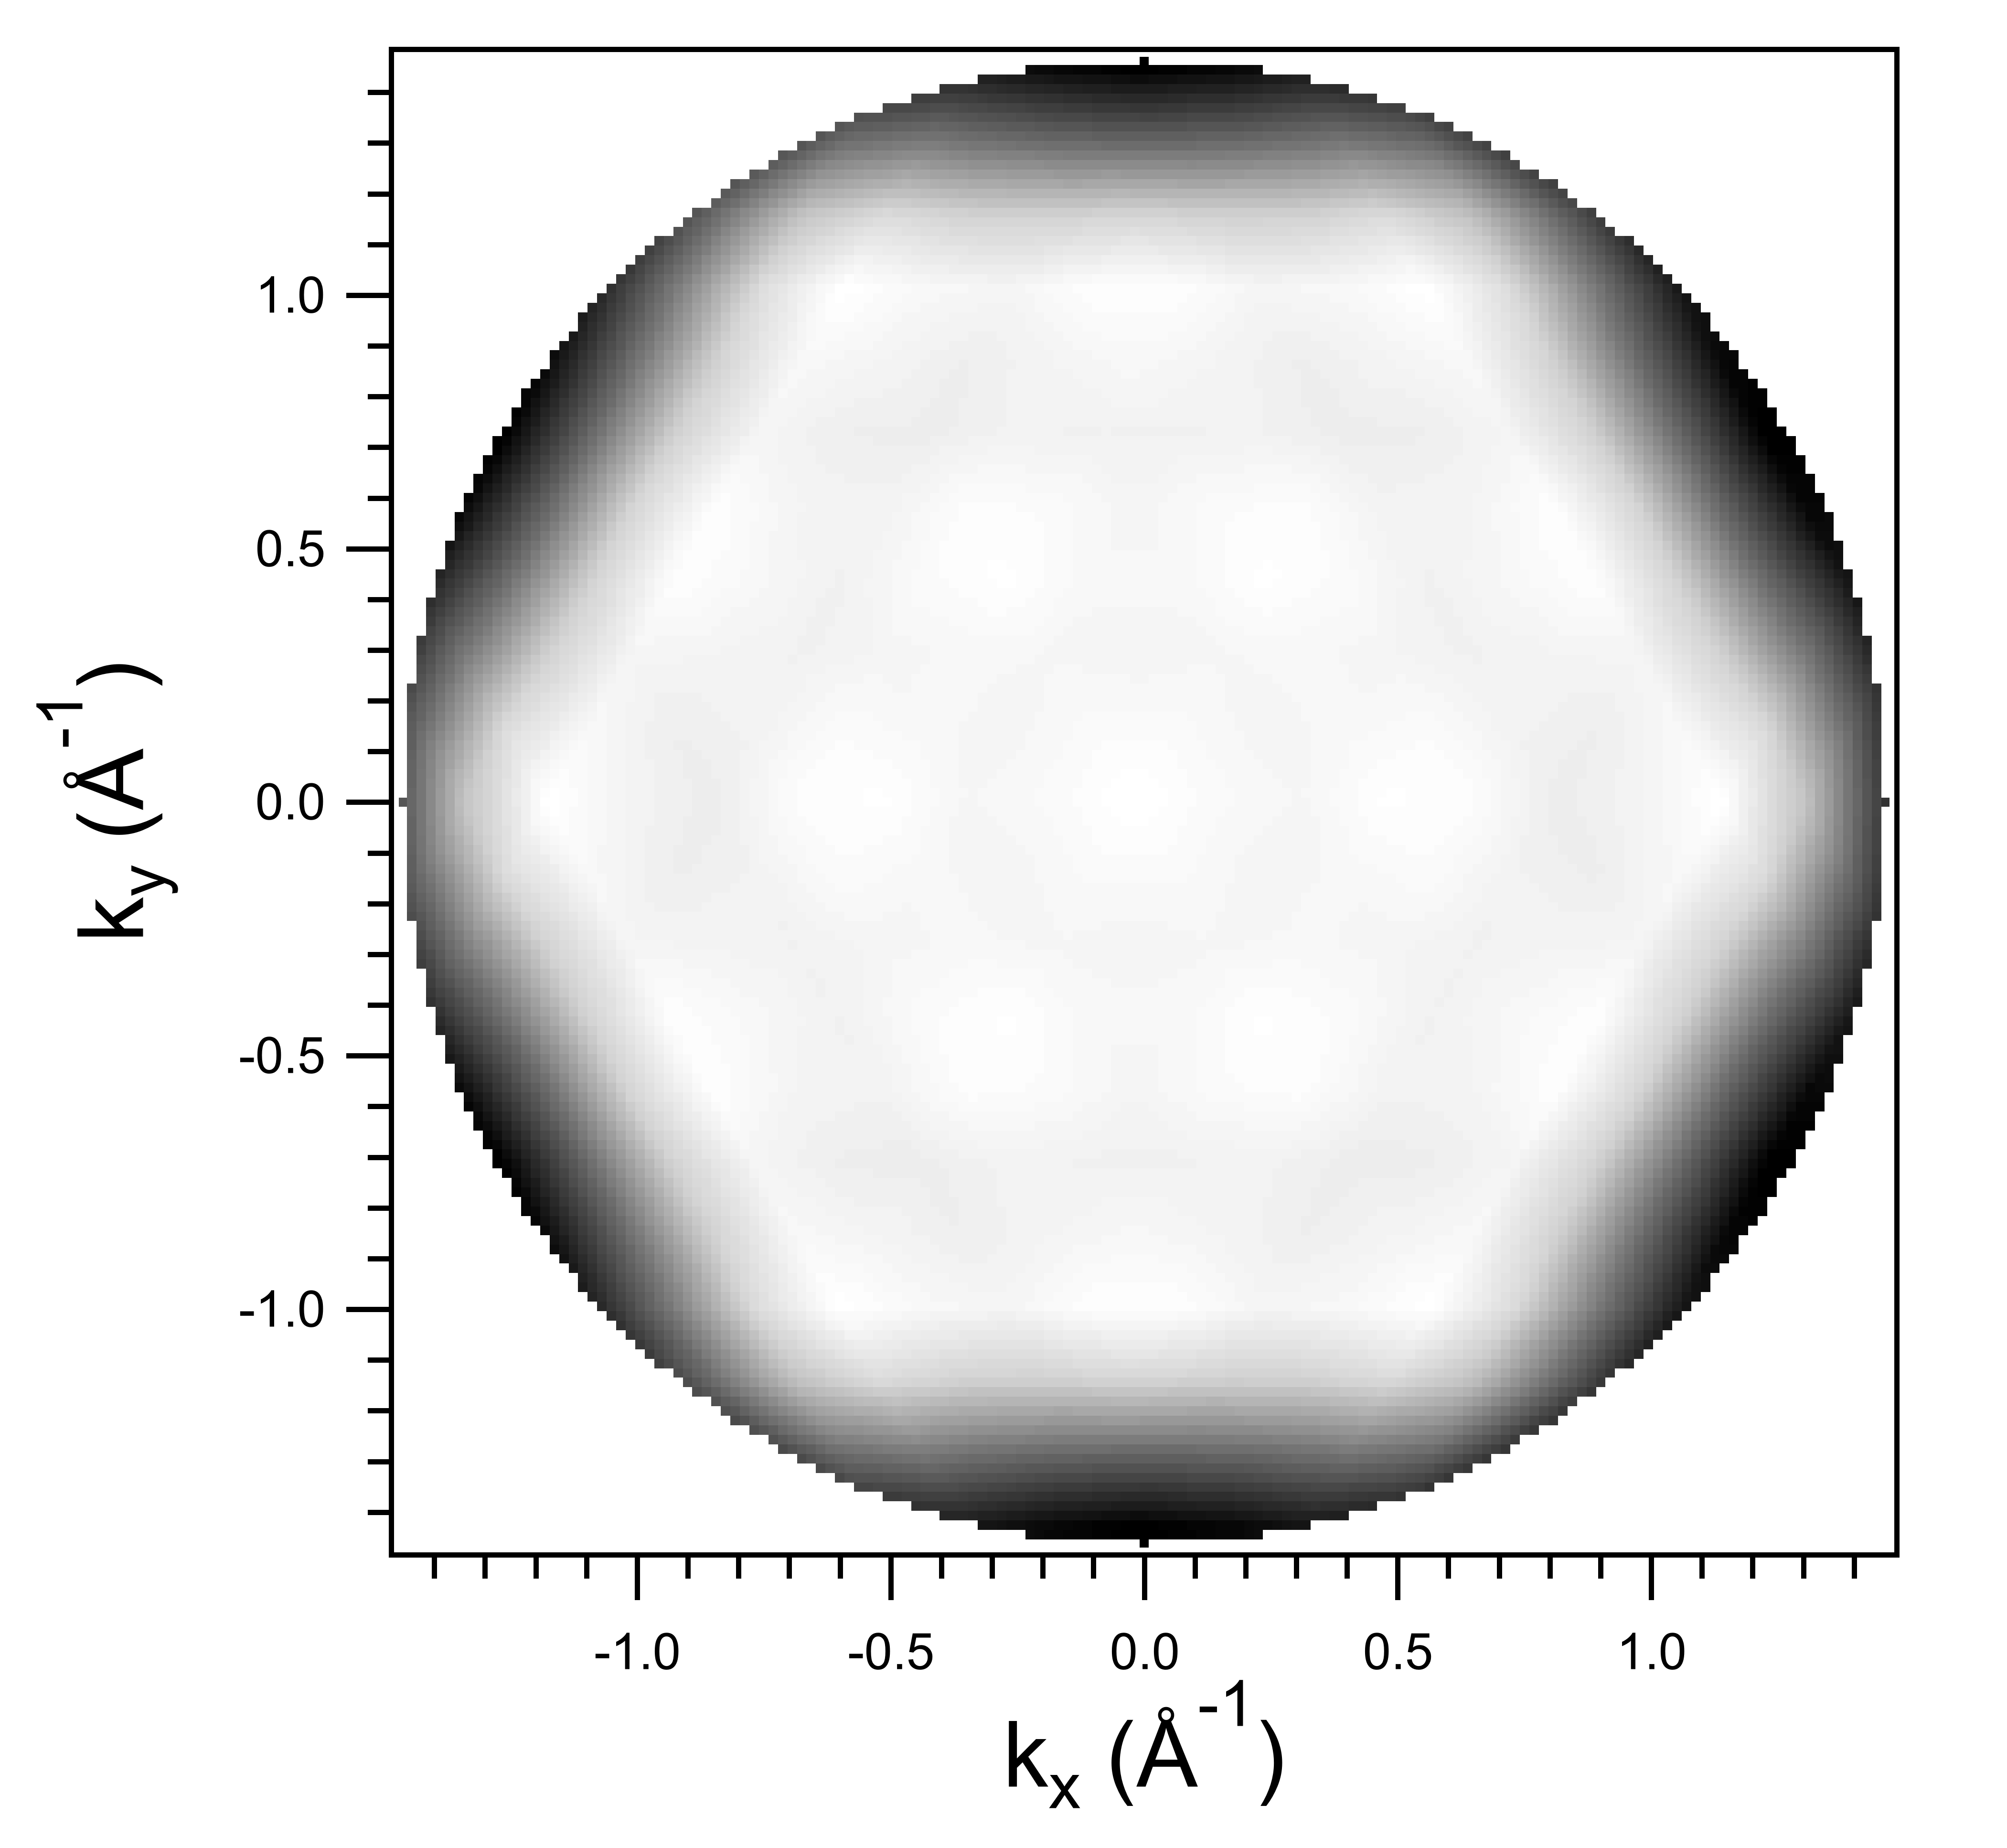
\includegraphics[height=4cm]{Au+5A/HOMO2_all_CT}
                    \subcaption{Berechnetes Theoriebild zum HOMO-2.}
                    \label{fig:MOT_Au+5A_theo_3}
                \end{subfigure}
                \caption{Zuordnung eines Bildes zu einem der Molekülorbitale. Theorie Oribtale mit Symmetrisierung zweimal um 120 Grad gedreht und zum Ursprungsbild addiert.}
                \label{fig:MOT_Au+5A}
            \end{figure}
            Winkelaufgelöste Bilder bei den entsprechenden Energien zeigen auch zusätzliche Merkmale im Bezug zum reinen Gold.
            Gemeinsam mit theoretischen Berechnungen aus der Dichtefunktionaltheorie lassen sich diese dann entsprechenden Molekülorbitalen zuordnen.
            Dies ist für einige Energien und Orbitale in \autoref{fig:MOT_Au+5A} geschehen.
            Dabei wurden die gemessenen wie auch berechneten Bilder entsprechend der Geometrie aus dem Beugungsbild \autoref{fig:LEED_Au+5A} jeweils um \SI{120}{\degree} gedreht und aufsummiert.
    
            Eine Zuordnung einer der markanten Elemente zu einem zuvor unbestzten Orbital, dem LUMO ist nicht zu erkennen.
            Es scheint also so als würden keine Elektronen zwischen Substrat und Molekül ausgetauscht werden. 
            Dies lässt sich auch aus der Literatur erkennen, dass sich bei den Anornung von Pentacene auf Gold um den Prozess der Physisorption handelt~\cite{5A_4}.
            Abwesenheit des LUMOs in den Spektren und Bildern muss aber nicht zwangsläufig auf die Physisorption hindeuten.
            So ist Pentacene auf Kupfer (111) chemisch adsorbiert und zeigt dennoch keine Anzeichen der Besetzung des LUMO~\cite{koch_adsorption-induced_2008}.

            \section{Sonstiges}
            \begin{itemize}
                \item Die mittlere freie Weglänge $\lambda$ ist die in der \SI{63}{\percent} der Elektronen Energieverlust erfahren \cite{vickerman_surface_2009}
                \item Durch den Vergleich von VB bei XPS und UPS sieht man Effekt ob von metallischem d (XPS) oder Liganden kommt (UPS - Intensitäten gleich ob metalisch oder Ligand) \cite{FeO_44}
            \end{itemize}

            \subsection{XMCD/XMLD}
            Neben der Abhänigkeit von der Photonenenergien ist die Absorption auch von der Polarisation des Lichts selbst abhängig.
            So lässt sich aus den Unterschieden der Absorptionsintensitäten für s- und p-polarisiertem Licht die Neigung von Molekülen auf der Oberfläche kalkulieren\cite{floreano_periodic_2008}.
            Ebenso wird durch die Ausrichtung der magetischen Momente die Orbitalstruktur ebenfalls in diese Richtung gestreckt.
            Nun kommt der Polarisationfaktor für den Photoemissionsstrom zu tragen.
            Sind Polarisation der Photonen und Orbitalgeometrie parallel gerichtet kommt es zur verstärkten Absorption, im Gegensatzt dazu, wenn diese senkrecht aufeinander stehen.
            Aus der Differenz der beiden Anteile ergibt sich dann das Signal der Röntgen linear magnetischer Dichroismus (XMLD, \textit{X-ray magnetic linear dichroism}).
            Dieser Effekt tritt für antiferromagnetisch wie auch für ferromagnetisch Materialien auf.
            Für zirkularpolarisiertes Licht ergibt sich aus dem Intensitätsunterschied der links- und rechtszirkularpolarisertem Licht die Magnetisierung für ferromagnetisch Materialien.
            Durch die unterschiedelichen Polarisationen wird die eine oder andere Spinsorte vermehrt angeregt.
            An der Fermikante sind nur Zustände einer gewissen Spinsorte unbesetz.
            Da ein Spinflip verboten ist, dienen diese Zustände als Detektor für den Spin der angeregten Elektronen~\cite{stohr_magnetism_2006}.

            \subsection{Wüstit}
            \begin{figure}
                \centering
                \begin{subfigure}[t]{0.48\textwidth}
                    \centering
                    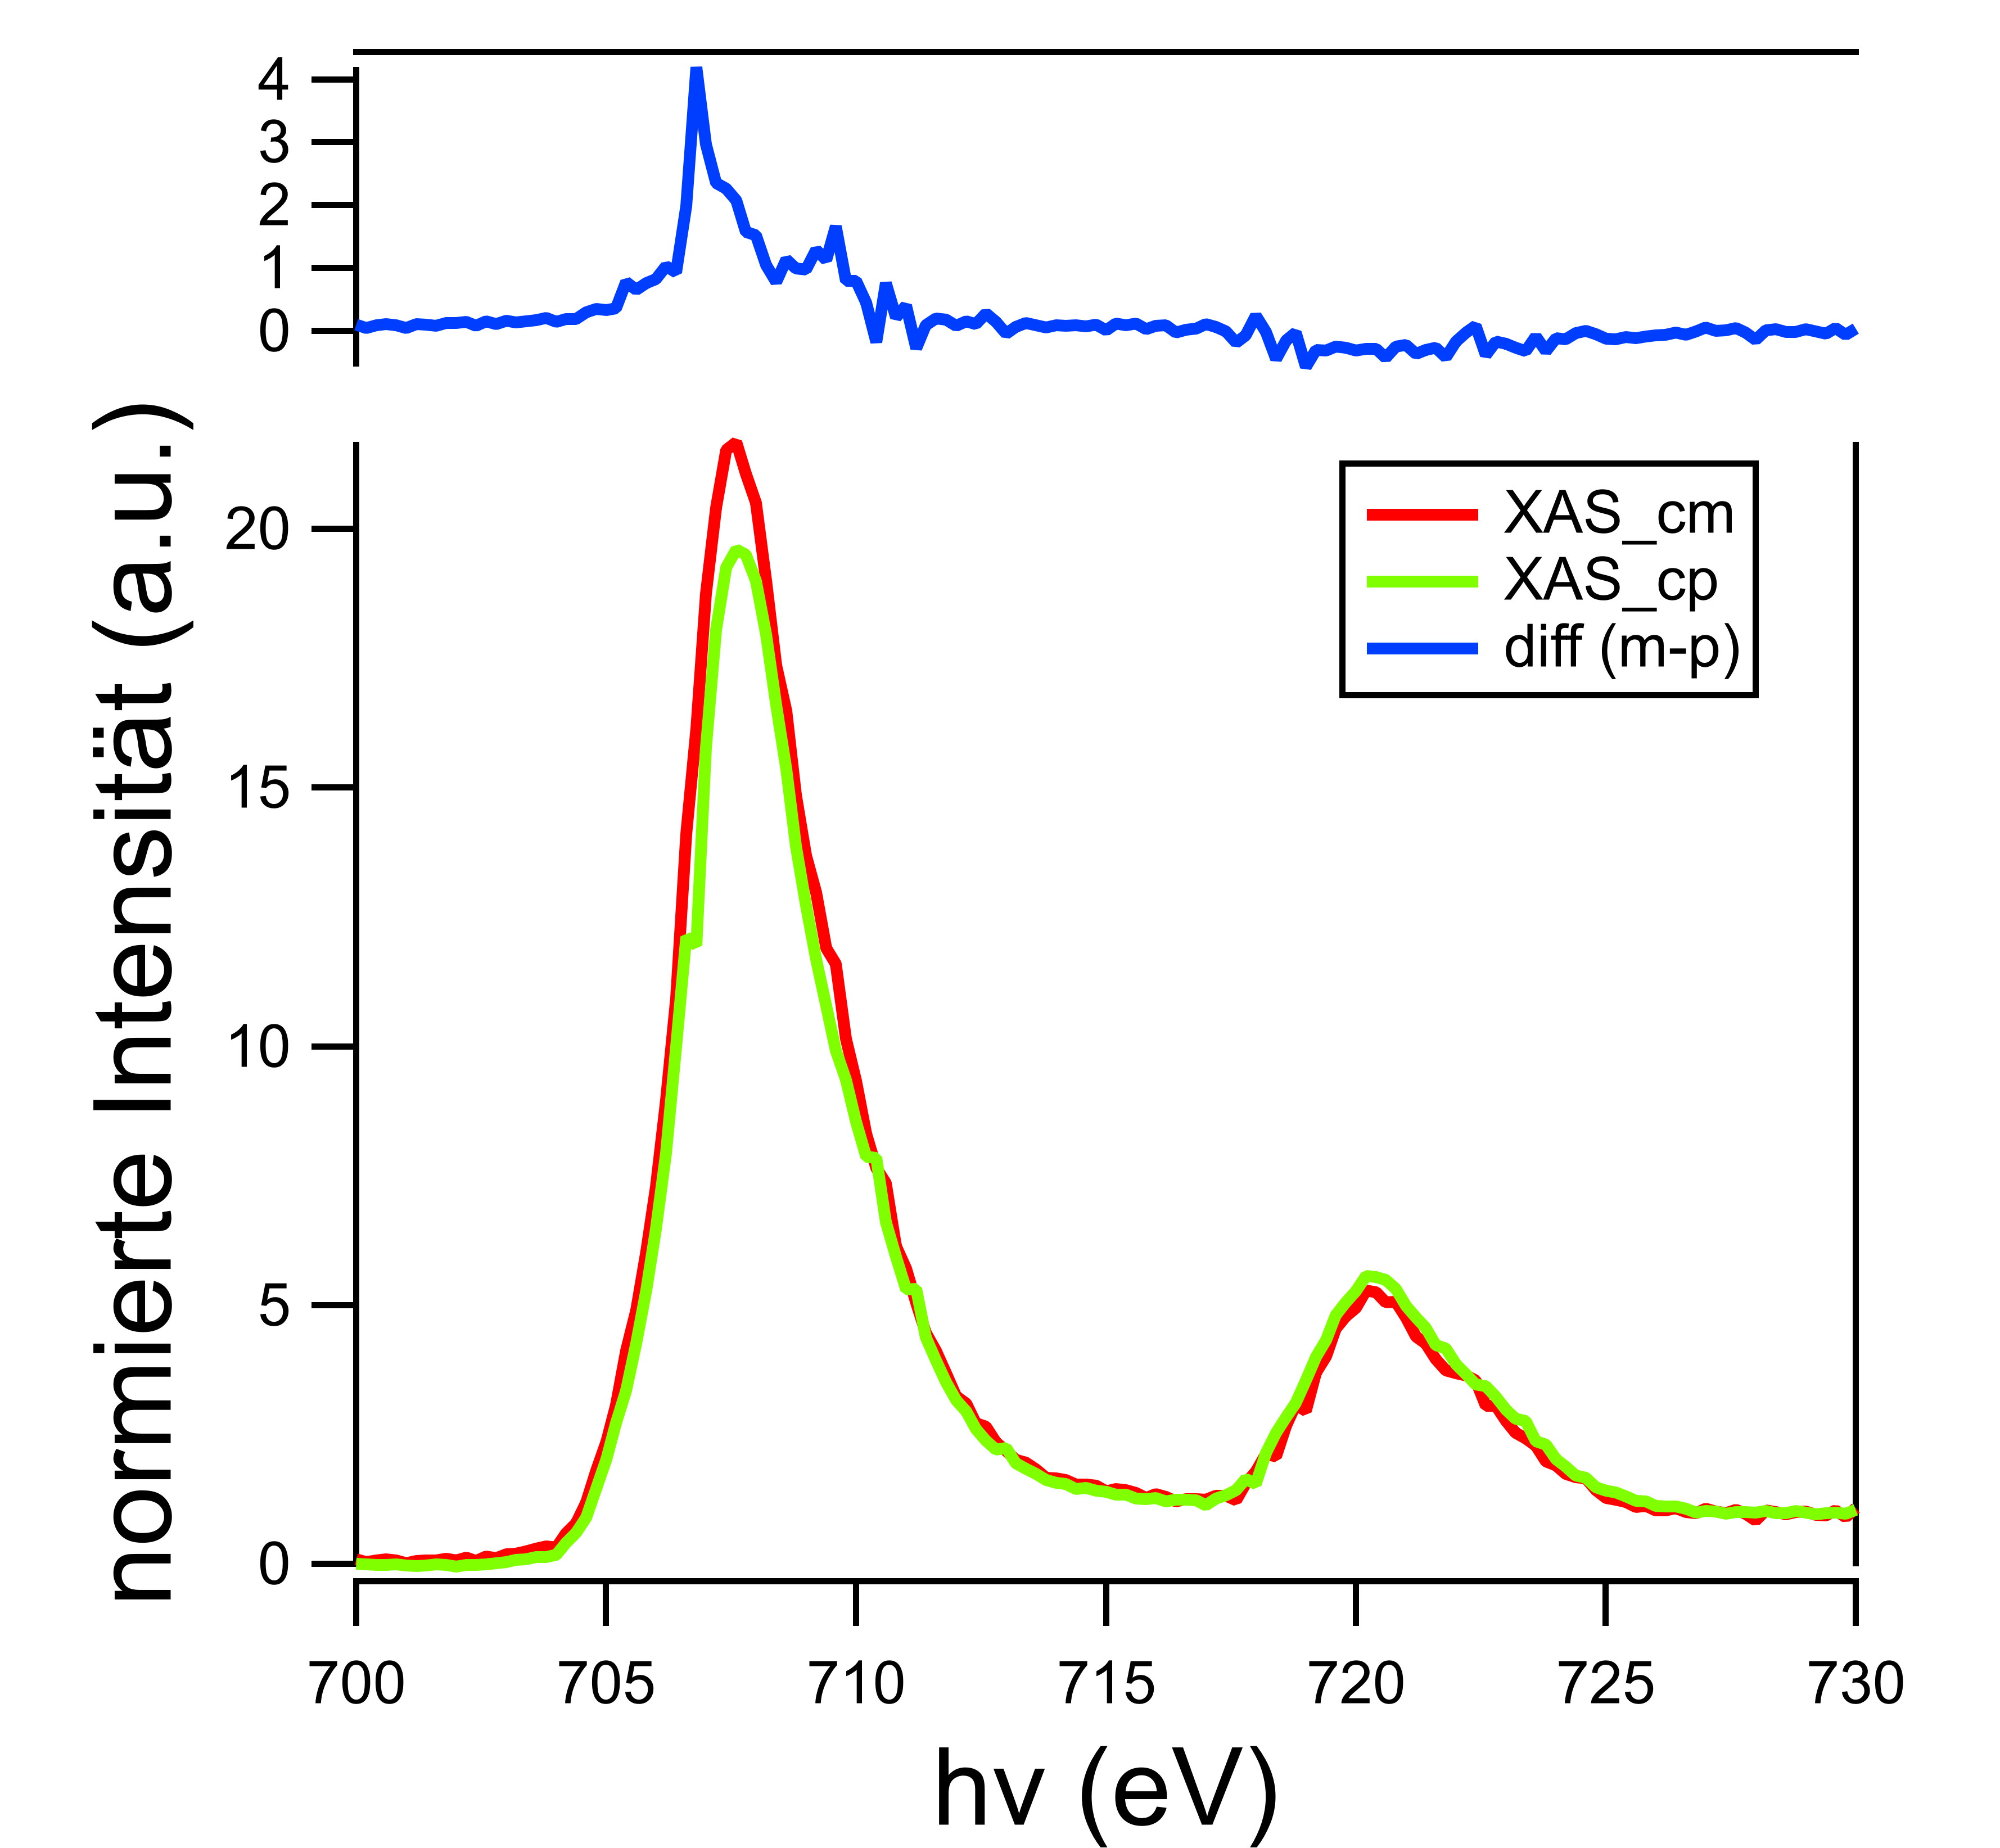
\includegraphics[height=5cm]{FeO/XMCD_FeO.png}
                    \caption{Spektren für links- und rechtzirkular polarisiertes Licht und ihre Differenz dem XMCD Signal.}
                    \label{fig:XMCD}
                \end{subfigure}
                \begin{subfigure}[t]{0.48\textwidth}
                    \centering
                    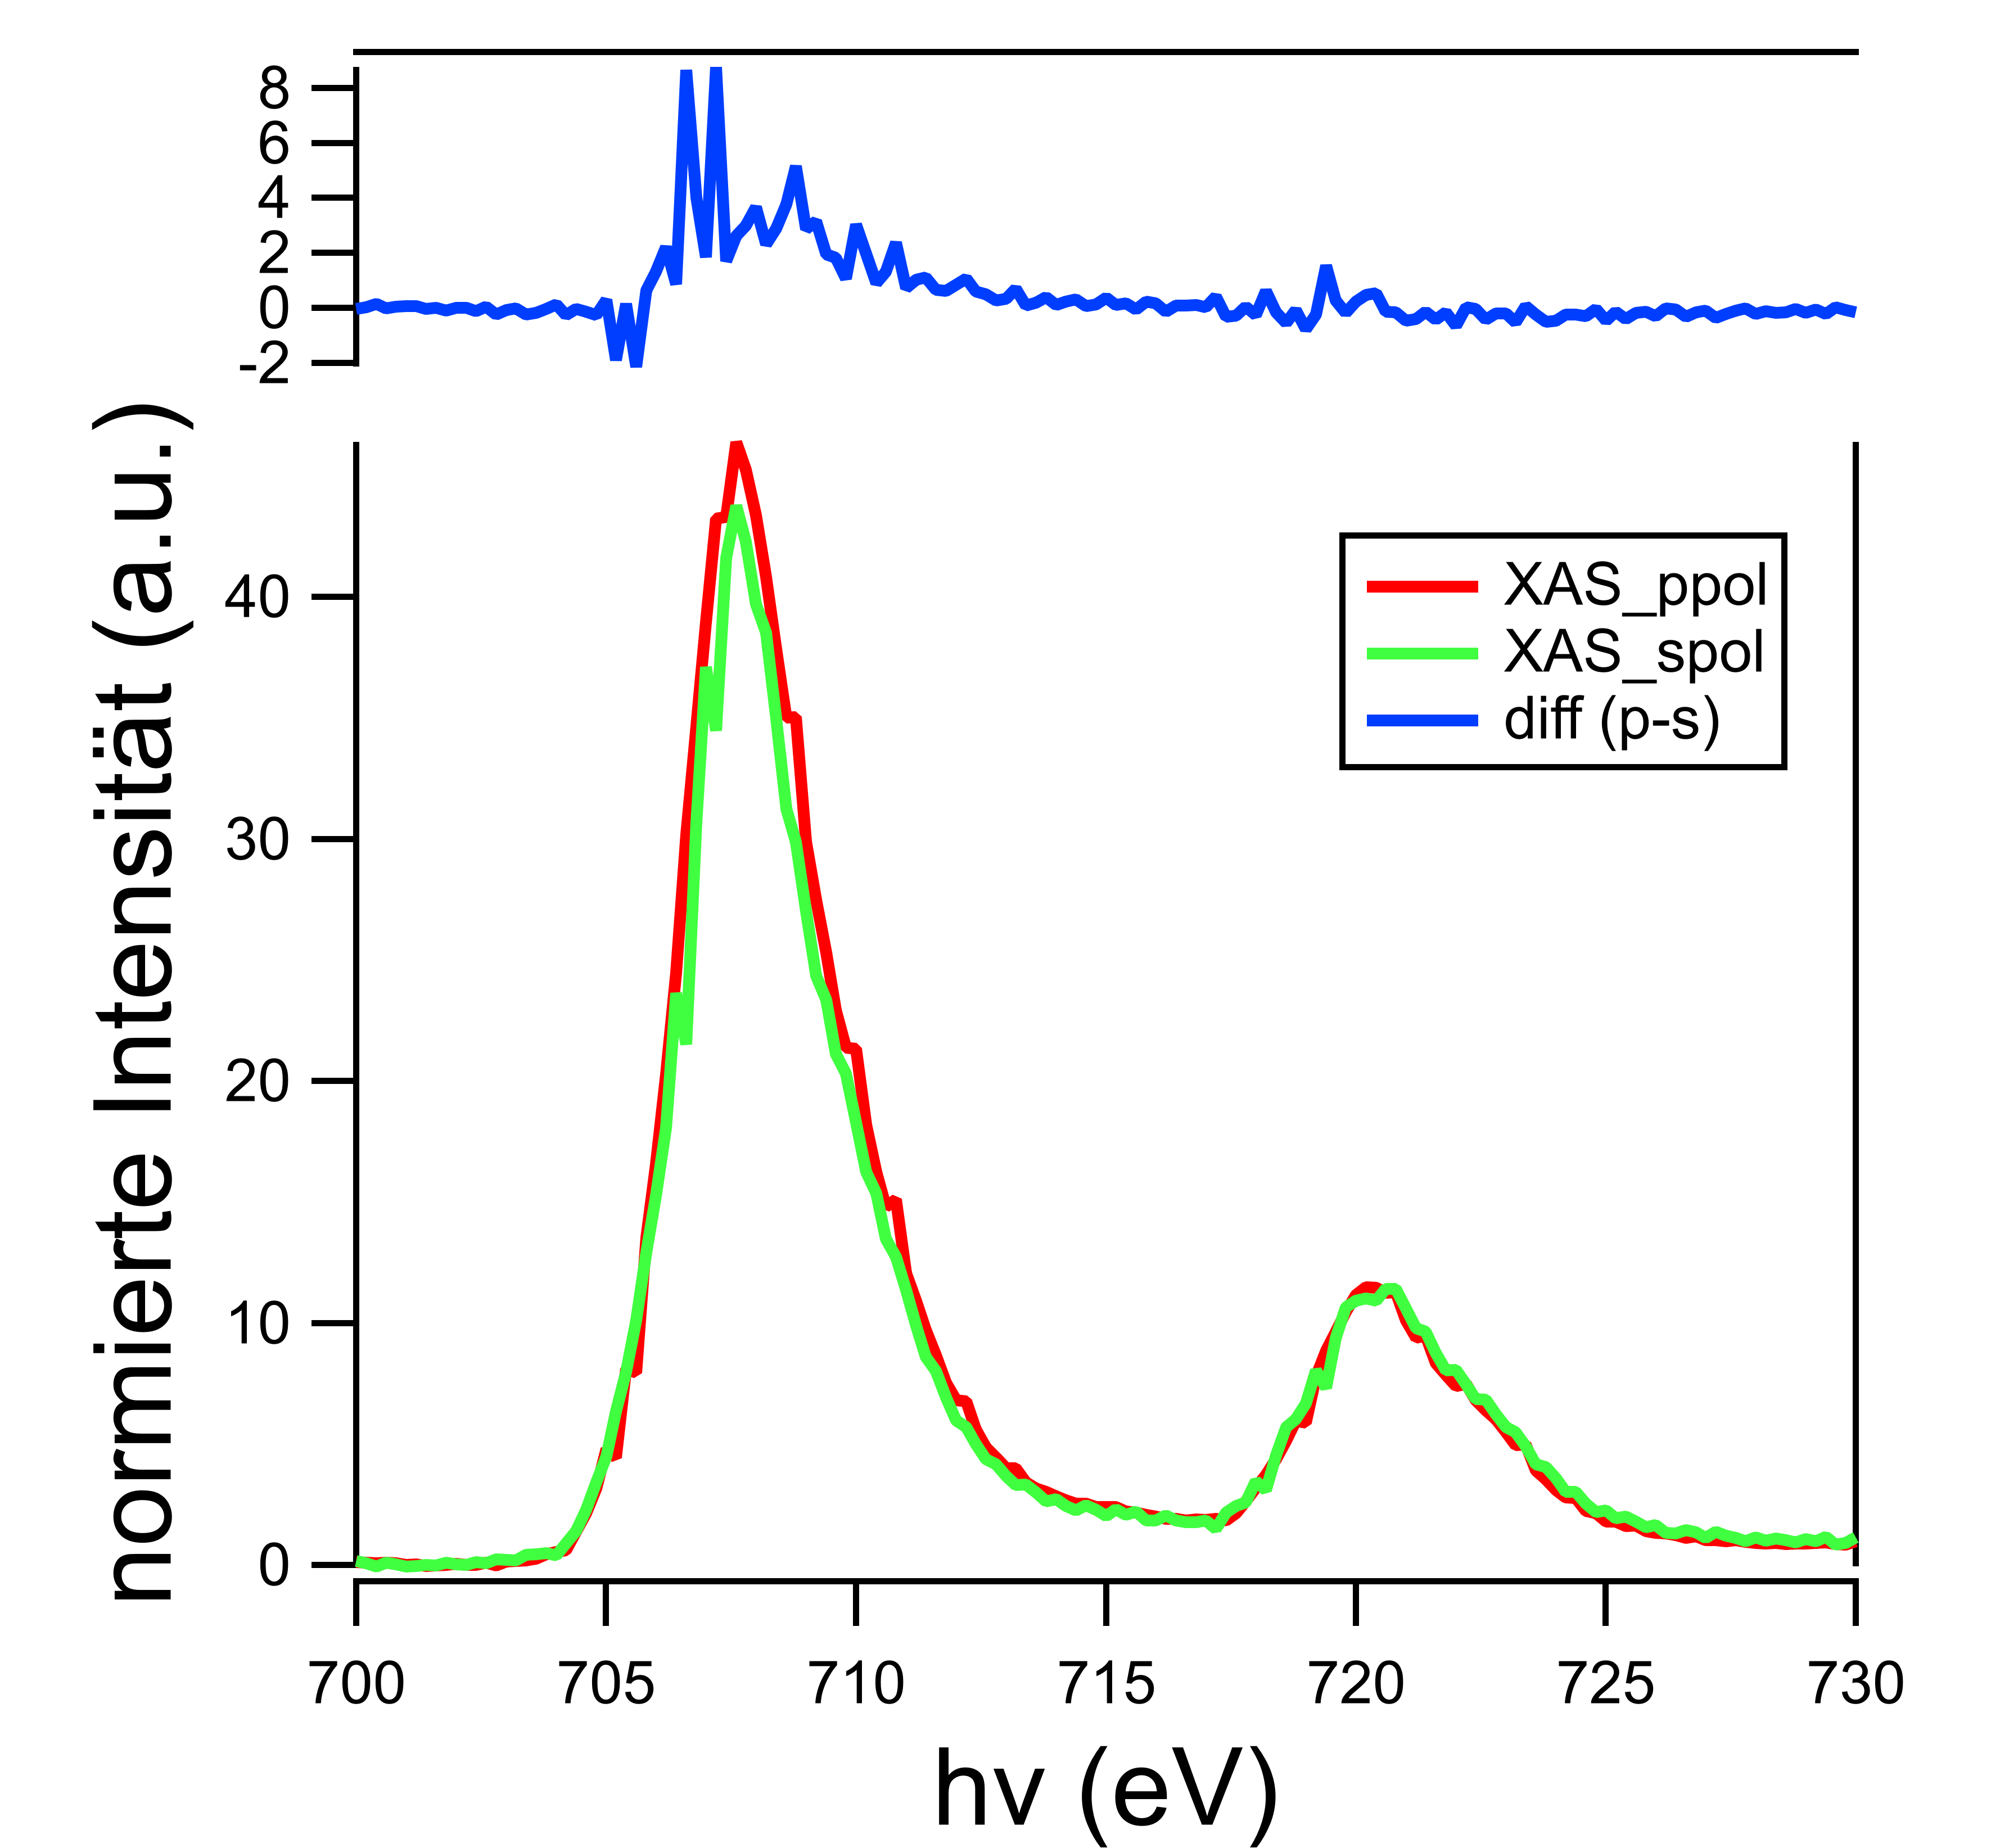
\includegraphics[height=5cm]{FeO/XMLD_FeO.png}
                    \caption{Spektren für s- und p- polarisiertes Licht, sowie dessen Differenz dem XMLD Signal.}
                    \label{fig:XMLD}
                \end{subfigure}
                \caption{Die verschiedenen XAS Messungen mit unterschiedlichen Polarisationen. Aus der Differenz ergeben sich dann die XMCD und XMLD Signale.}
                \label{fig:XAS_FeO}
            \end{figure}
            Mit Hilfe des magnetischen Röntgen-Zirkular-Dikorismus und magnetischen Röntgen-Linear-Dikorismus lassen sich die magnetischen Eigeschaften des Substrates untersuchen.
            Beide Spektren der Röntgenabsorptionsmessungen sind in \autoref{fig:XAS_FeO} zu sehen.
            \begin{itemize}
                \item Das XMCD Signal sollte für L3 und L2 umegkehrt sein, wenn es Ferromagnetisch ist, Signal lässt sich aber nur bei L3 erkennen.
                \item Auch XMLD für Antiferromagnetismus auf Grund der nicht spärischen Oribtale durch die Spin-Bahn-Kopplung (Spins ausgerichtet) \cite{stohr_magnetism_2006} - kann auch eben sein, dass die Spins nicht ausgerichtet waren. T war unter Neel Temperatur.
                \item Eventuell kein XMLD Signal, falls Probe nicht geordnet oder viele Domänen aufweist. Die Easy-Axis des Fe lag auch genau 45° zu p und s.
                \item Kleine XMLD Effekte können auch durch die Liganden zu stande kommen, da diese ja auch das Orbital verformen können (besser T abhänig messen)
                \item Warum kein XMCD und XMLD Signal? Es bilden sich Domänen mit einer Größe von \SIrange{50}{500}{\nano\meter} aus. Diese müssen erst durch ein hinreichend großes Feld ausgerichtet werden. Ansonsten haben die Domänen alle Magnetisierungen in unterschiedliche Richtungen. \cite{cornell_iron_2003}

            \end{itemize}

\backmatter
\printbibliography

%\cleardoublepage
% \thispagestyle{empty}
\section*{Eidesstattliche Versicherung}
Ich versichere hiermit an Eides statt, dass ich die vorliegende Abschlussarbeit mit dem Titel \enquote{\thetitle} selbstständig und ohne unzulässige fremde Hilfe erbracht habe.
Ich habe keine anderen als die angegebenen Quellen und Hilfsmittel benutzt, sowie wörtliche und sinngemäße Zitate kenntlich gemacht. 
Die Arbeit hat in gleicher oder ähnlicher Form noch keiner Prüfungsbehörde vorgelegen.

\vspace*{1cm}\noindent
\begin{center}
  \begin{tabular}{@{}p{0.4\textwidth}@{\hspace{0.15\textwidth}}p{0.4\textwidth}@{}}
  \rule{\linewidth}{0.25pt}& \rule{\linewidth}{0.25pt}\\
  Ort, Datum & Unterschrift
  \end{tabular}
\end{center}

\subsection*{Belehrung}
Wer vorsätzlich gegen eine die Täuschung über Prüfungsleistungen betreffende Regelung einer Hochschulprüfungsordnung verstößt, handelt ordnungswidrig.
Die Ordnungswidrigkeit kann mit einer Geldbuße von bis zu \SI[round-mode=places, round-precision=2]{50000}{€} geahndet werden. 
Zuständige Verwaltungsbehörde für die Verfolgung und Ahndung von Ordnungswidrigkeiten ist der Kanzler/die Kanzlerin der Technischen Universität Dortmund. 
Im Falle eines mehrfachen oder sonstigen schwerwiegenden Täuschungsversuches kann der Prüfling zudem exmatrikuliert werden \mbox{(\S\,63 Abs. 5 Hochschulgesetz --HG--).}

Die Abgabe einer falschen Versicherung an Eides statt wird mit Freiheitsstrafe bis zu 3 Jahren oder mit Geldstrafe bestraft.

Die Technische Universität Dortmund wird ggf.\ elektronische Vergleichswerkzeuge (wie z.\,B.\ die Software \enquote{turnitin}) zur Überprüfung von Ordnungswidrigkeiten in Prüfungsverfahren nutzen. \\[\baselineskip]

\noindent Die oben stehende Belehrung habe ich zur Kenntnis genommen.\\[1cm]
\begin{center}
\begin{tabular}{@{}p{0.4\textwidth}@{\hspace{0.15\textwidth}}p{0.4\textwidth}@{}}
\rule{\linewidth}{0.25pt}& \rule{\linewidth}{0.25pt}\\
Ort, Datum & Unterschrift
\end{tabular}
\end{center}

\end{document}
